\documentclass[twoside]{book}

% Packages required by doxygen
\usepackage{fixltx2e}
\usepackage{calc}
\usepackage{doxygen}
\usepackage[export]{adjustbox} % also loads graphicx
\usepackage{graphicx}
\usepackage[utf8]{inputenc}
\usepackage{makeidx}
\usepackage{multicol}
\usepackage{multirow}
\PassOptionsToPackage{warn}{textcomp}
\usepackage{textcomp}
\usepackage[nointegrals]{wasysym}
\usepackage[table]{xcolor}

% NLS support packages
\usepackage[spanish]{babel}
% Font selection
\usepackage[T1]{fontenc}
\usepackage[scaled=.90]{helvet}
\usepackage{courier}
\usepackage{amssymb}
\usepackage{sectsty}
\renewcommand{\familydefault}{\sfdefault}
\allsectionsfont{%
  \fontseries{bc}\selectfont%
  \color{darkgray}%
}
\renewcommand{\DoxyLabelFont}{%
  \fontseries{bc}\selectfont%
  \color{darkgray}%
}
\newcommand{\+}{\discretionary{\mbox{\scriptsize$\hookleftarrow$}}{}{}}

% Page & text layout
\usepackage{geometry}
\geometry{%
  a4paper,%
  top=2.5cm,%
  bottom=2.5cm,%
  left=2.5cm,%
  right=2.5cm%
}
\tolerance=750
\hfuzz=15pt
\hbadness=750
\setlength{\emergencystretch}{15pt}
\setlength{\parindent}{0cm}
\setlength{\parskip}{3ex plus 2ex minus 2ex}
\makeatletter
\renewcommand{\paragraph}{%
  \@startsection{paragraph}{4}{0ex}{-1.0ex}{1.0ex}{%
    \normalfont\normalsize\bfseries\SS@parafont%
  }%
}
\renewcommand{\subparagraph}{%
  \@startsection{subparagraph}{5}{0ex}{-1.0ex}{1.0ex}{%
    \normalfont\normalsize\bfseries\SS@subparafont%
  }%
}
\makeatother

% Headers & footers
\usepackage{fancyhdr}
\pagestyle{fancyplain}
\fancyhead[LE]{\fancyplain{}{\bfseries\thepage}}
\fancyhead[CE]{\fancyplain{}{}}
\fancyhead[RE]{\fancyplain{}{\bfseries\leftmark}}
\fancyhead[LO]{\fancyplain{}{\bfseries\rightmark}}
\fancyhead[CO]{\fancyplain{}{}}
\fancyhead[RO]{\fancyplain{}{\bfseries\thepage}}
\fancyfoot[LE]{\fancyplain{}{}}
\fancyfoot[CE]{\fancyplain{}{}}
\fancyfoot[RE]{\fancyplain{}{\bfseries\scriptsize Generado por Doxygen }}
\fancyfoot[LO]{\fancyplain{}{\bfseries\scriptsize Generado por Doxygen }}
\fancyfoot[CO]{\fancyplain{}{}}
\fancyfoot[RO]{\fancyplain{}{}}
\renewcommand{\footrulewidth}{0.4pt}
\renewcommand{\chaptermark}[1]{%
  \markboth{#1}{}%
}
\renewcommand{\sectionmark}[1]{%
  \markright{\thesection\ #1}%
}

% Indices & bibliography
\usepackage{natbib}
\usepackage[titles]{tocloft}
\setcounter{tocdepth}{3}
\setcounter{secnumdepth}{5}
\makeindex

% Hyperlinks (required, but should be loaded last)
\usepackage{ifpdf}
\ifpdf
  \usepackage[pdftex,pagebackref=true]{hyperref}
\else
  \usepackage[ps2pdf,pagebackref=true]{hyperref}
\fi
\hypersetup{%
  colorlinks=true,%
  linkcolor=blue,%
  citecolor=blue,%
  unicode%
}

% Custom commands
\newcommand{\clearemptydoublepage}{%
  \newpage{\pagestyle{empty}\cleardoublepage}%
}

\usepackage{caption}
\captionsetup{labelsep=space,justification=centering,font={bf},singlelinecheck=off,skip=4pt,position=top}

%===== C O N T E N T S =====

\begin{document}

% Titlepage & ToC
\hypersetup{pageanchor=false,
             bookmarksnumbered=true,
             pdfencoding=unicode
            }
\pagenumbering{roman}
\begin{titlepage}
\vspace*{7cm}
\begin{center}%
{\Large Práctica P\+R\+O2\+: Tree\+K\+EA\textquotesingle{}. \\[1ex]\large version 1.\+0 2-\/mayo-\/2018 }\\
\vspace*{1cm}
{\large Generado por Doxygen 1.8.11}\\
\end{center}
\end{titlepage}
\clearemptydoublepage
\tableofcontents
\clearemptydoublepage
\pagenumbering{arabic}
\hypersetup{pageanchor=true}

%--- Begin generated contents ---
\chapter{Diseño modular\+: Tree\+K\+EA}
\label{index}\hypertarget{index}{}Tendremos un programa con un menú de opciones que se encuentra en \hyperlink{program_8cc}{program.\+cc} para gestionar un almacen con salas y un inventario sobre todos sus productos. Las clases utilizadas son\+: {\itshape \hyperlink{class_almacen}{Almacen}}, {\itshape \hyperlink{class_inventario}{Inventario}} y {\itshape \hyperlink{class_sala}{Sala}}.


\begin{DoxyItemize}
\item Para que el diagrama modular quede bien se han hecho \char`\"{}includes\char`\"{} redundantes. 
\end{DoxyItemize}
\chapter{Índice de clases}
\section{Lista de clases}
Lista de las clases, estructuras, uniones e interfaces con una breve descripción\+:\begin{DoxyCompactList}
\item\contentsline{section}{\hyperlink{class_almacen}{Almacen} \\*Representa una almacen con varias salas estructuradas en forma de arbol }{\pageref{class_almacen}}{}
\item\contentsline{section}{\hyperlink{class_inventario}{Inventario} \\*Representa el inventario de los productos de un almacen }{\pageref{class_inventario}}{}
\item\contentsline{section}{\hyperlink{class_sala}{Sala} \\*Representa una sala de un numero de filas y columnas }{\pageref{class_sala}}{}
\end{DoxyCompactList}

\chapter{Indice de archivos}
\section{Lista de archivos}
Lista de todos los archivos con descripciones breves\+:\begin{DoxyCompactList}
\item\contentsline{section}{\hyperlink{_almacen_8cc}{Almacen.\+cc} \\*Código de la clase \hyperlink{class_almacen}{Almacen} }{\pageref{_almacen_8cc}}{}
\item\contentsline{section}{\hyperlink{_almacen_8hh}{Almacen.\+hh} \\*Especificación de la clase \hyperlink{class_almacen}{Almacen} }{\pageref{_almacen_8hh}}{}
\item\contentsline{section}{\hyperlink{_inventario_8cc}{Inventario.\+cc} \\*Código de la clase \hyperlink{class_inventario}{Inventario} }{\pageref{_inventario_8cc}}{}
\item\contentsline{section}{\hyperlink{_inventario_8hh}{Inventario.\+hh} \\*Especificación de la clase \hyperlink{class_inventario}{Inventario} }{\pageref{_inventario_8hh}}{}
\item\contentsline{section}{\hyperlink{program_8cc}{program.\+cc} \\*Programa principal para la practica {\itshape Tree\+K\+EA} }{\pageref{program_8cc}}{}
\item\contentsline{section}{\hyperlink{_sala_8cc}{Sala.\+cc} \\*Código de la clase \hyperlink{class_sala}{Sala} }{\pageref{_sala_8cc}}{}
\item\contentsline{section}{\hyperlink{_sala_8hh}{Sala.\+hh} \\*Especificación de la clase \hyperlink{class_sala}{Sala} }{\pageref{_sala_8hh}}{}
\end{DoxyCompactList}

\chapter{Documentación de las clases}
\hypertarget{class_almacen}{}\section{Referencia de la Clase Almacen}
\label{class_almacen}\index{Almacen@{Almacen}}


Representa una almacen con varias salas estructuradas en forma de arbol.  


\subsection*{Métodos públicos}
\begin{DoxyCompactItemize}
\item 
\hyperlink{class_almacen_a68a6084d5775d391c52d4825072a0612}{Almacen} ()
\begin{DoxyCompactList}\small\item\em Creadora por defecto. \end{DoxyCompactList}\item 
\hyperlink{class_almacen_ae5ed0e91d616199b8dbdc1f8780a7efb}{Almacen} (int n)
\begin{DoxyCompactList}\small\item\em Creadora por numero de salas. \end{DoxyCompactList}\item 
void \hyperlink{class_almacen_a5532f34bea73002793d637b2031698c8}{poner\+\_\+items} (int id, string producto, int cantidad, \hyperlink{class_inventario}{Inventario} \&i)
\begin{DoxyCompactList}\small\item\em Coloca una cantidad de productos en la sala \char`\"{}id\char`\"{}. \end{DoxyCompactList}\item 
void \hyperlink{class_almacen_ab28cb9537ce54d2c67d1c85f69c2e09c}{quitar\+\_\+items} (int id, string producto, int cantidad, \hyperlink{class_inventario}{Inventario} \&i)
\begin{DoxyCompactList}\small\item\em Coloca una cantidad de productos en la sala \char`\"{}id\char`\"{}. \end{DoxyCompactList}\item 
void \hyperlink{class_almacen_a9e266b71d6ab186830abb7b3a367ecc0}{distribuir} (string producto, int cantidad, \hyperlink{class_inventario}{Inventario} \&i)
\begin{DoxyCompactList}\small\item\em Operacion de distribucion. \end{DoxyCompactList}\item 
void \hyperlink{class_almacen_a9b0a893ac5ea4774bd362e297b2c3770}{compactar} (int id)
\begin{DoxyCompactList}\small\item\em Compactadora de sala especifica. \end{DoxyCompactList}\item 
void \hyperlink{class_almacen_a9e27219c735096dab9d5d3edc2ae2012}{reorganizar} (int id)
\begin{DoxyCompactList}\small\item\em Reorganizadora de sala especifica. \end{DoxyCompactList}\item 
void \hyperlink{class_almacen_a477373756d8671d1acef1c7d84a926a9}{redimensionar} (int id, int f, int c)
\begin{DoxyCompactList}\small\item\em Redimensionadora de sala especifica. \end{DoxyCompactList}\item 
void \hyperlink{class_almacen_af3a411fa6f4e0d5b327697bdcd08c41c}{consultar\+\_\+pos} (int id, int f, int c) const 
\begin{DoxyCompactList}\small\item\em Consultora por posicion y sala. \end{DoxyCompactList}\item 
void \hyperlink{class_almacen_a4ed23c4daa30f40be6fb8986ab04cbef}{inisalas} ()
\begin{DoxyCompactList}\small\item\em Da tamaño a cada una de las salas del almacen. \end{DoxyCompactList}\item 
void \hyperlink{class_almacen_aee1a1a170d9712b5988692cb93791a4c}{creabtree} ()
\begin{DoxyCompactList}\small\item\em Inicializa la estructura del almacen. \end{DoxyCompactList}\item 
void \hyperlink{class_almacen_a139a466ffe4ed01057a19607e1c4d437}{escribir} (int id) const 
\begin{DoxyCompactList}\small\item\em Operacion de escritura de la sala con identificador \char`\"{}id\char`\"{}. \end{DoxyCompactList}\end{DoxyCompactItemize}
\subsection*{Métodos privados estáticos}
\begin{DoxyCompactItemize}
\item 
static void \hyperlink{class_almacen_ab17f45bbf11a4c178ee4acefd6d085eb}{btree} (Bin\+Tree$<$ int $>$ \&b)
\begin{DoxyCompactList}\small\item\em Operacion de lectura de identificadores de salas. \end{DoxyCompactList}\item 
static int \hyperlink{class_almacen_a0a613fcb43d66dea5965a3588c66110d}{distr} (const Bin\+Tree$<$ int $>$ \&b, vector$<$ \hyperlink{class_sala}{Sala} $>$ \&\hyperlink{class_almacen_a5c60aa6a014eb6a96a2f5c6fb9a83e52}{salas}, int cantidad, string producto)
\begin{DoxyCompactList}\small\item\em Operacion de distribucion. \end{DoxyCompactList}\end{DoxyCompactItemize}
\subsection*{Atributos privados}
\begin{DoxyCompactItemize}
\item 
Bin\+Tree$<$ int $>$ \hyperlink{class_almacen_a32ee5ed02255216a7ec6ac90e5d2030b}{alm}
\begin{DoxyCompactList}\small\item\em Estructura de las salas en el almacen. \end{DoxyCompactList}\item 
vector$<$ \hyperlink{class_sala}{Sala} $>$ \hyperlink{class_almacen_a5c60aa6a014eb6a96a2f5c6fb9a83e52}{salas}
\begin{DoxyCompactList}\small\item\em Vector que contiene cada una de las salas del almacen. \end{DoxyCompactList}\end{DoxyCompactItemize}


\subsection{Descripción detallada}
Representa una almacen con varias salas estructuradas en forma de arbol. 

Desde cada sala puedes acceder a otras 2, una por la derecha, u otra por la izquierda o a ninguna. 

Definición en la línea 17 del archivo Almacen.\+hh.



\subsection{Documentación del constructor y destructor}
\index{Almacen@{Almacen}!Almacen@{Almacen}}
\index{Almacen@{Almacen}!Almacen@{Almacen}}
\subsubsection[{\texorpdfstring{Almacen()}{Almacen()}}]{\setlength{\rightskip}{0pt plus 5cm}Almacen\+::\+Almacen (
\begin{DoxyParamCaption}
{}
\end{DoxyParamCaption}
)}\hypertarget{class_almacen_a68a6084d5775d391c52d4825072a0612}{}\label{class_almacen_a68a6084d5775d391c52d4825072a0612}


Creadora por defecto. 

Se ejecuta automáticamente al declarar un almacen. \begin{DoxyPrecond}{Precondición}
{\itshape cierto} 
\end{DoxyPrecond}
\begin{DoxyPostcond}{Postcondición}
El resultado es una almacen sin salas 
\end{DoxyPostcond}
\begin{DoxyParagraph}{Coste}
Constante 
\end{DoxyParagraph}


Definición en la línea 39 del archivo Almacen.\+cc.


\begin{DoxyCode}
39                 \{
40     \hyperlink{class_almacen_a5c60aa6a014eb6a96a2f5c6fb9a83e52}{salas} = vector <Sala> (0);
41 \}
\end{DoxyCode}
\index{Almacen@{Almacen}!Almacen@{Almacen}}
\index{Almacen@{Almacen}!Almacen@{Almacen}}
\subsubsection[{\texorpdfstring{Almacen(int n)}{Almacen(int n)}}]{\setlength{\rightskip}{0pt plus 5cm}Almacen\+::\+Almacen (
\begin{DoxyParamCaption}
\item[{int}]{n}
\end{DoxyParamCaption}
)}\hypertarget{class_almacen_ae5ed0e91d616199b8dbdc1f8780a7efb}{}\label{class_almacen_ae5ed0e91d616199b8dbdc1f8780a7efb}


Creadora por numero de salas. 

Permite crear un almacen con un numero de salas \begin{DoxyPrecond}{Precondición}
El valor de n es un numero natual 
\end{DoxyPrecond}
\begin{DoxyPostcond}{Postcondición}
El resultado es un almacen con n salas 
\end{DoxyPostcond}
\begin{DoxyParagraph}{Coste}
Lineal respecto a n 
\end{DoxyParagraph}


Definición en la línea 43 del archivo Almacen.\+cc.


\begin{DoxyCode}
43                       \{
44     \hyperlink{class_almacen_a5c60aa6a014eb6a96a2f5c6fb9a83e52}{salas} = vector<Sala>(n);
45 \}
\end{DoxyCode}


\subsection{Documentación de las funciones miembro}
\index{Almacen@{Almacen}!btree@{btree}}
\index{btree@{btree}!Almacen@{Almacen}}
\subsubsection[{\texorpdfstring{btree(\+Bin\+Tree$<$ int $>$ \&b)}{btree(BinTree< int > &b)}}]{\setlength{\rightskip}{0pt plus 5cm}void Almacen\+::btree (
\begin{DoxyParamCaption}
\item[{Bin\+Tree$<$ int $>$ \&}]{b}
\end{DoxyParamCaption}
)\hspace{0.3cm}{\ttfamily [static]}, {\ttfamily [private]}}\hypertarget{class_almacen_ab17f45bbf11a4c178ee4acefd6d085eb}{}\label{class_almacen_ab17f45bbf11a4c178ee4acefd6d085eb}


Operacion de lectura de identificadores de salas. 

\begin{DoxyPrecond}{Precondición}
b esta vacio. 
\end{DoxyPrecond}
\begin{DoxyPostcond}{Postcondición}
El parametro implicito contiene identificadores de salas ordenado de forma jerarquizada. 
\end{DoxyPostcond}
\begin{DoxyParagraph}{Coste}
Lineal respecto al numero de salas del almacen. 
\end{DoxyParagraph}


Definición en la línea 6 del archivo Almacen.\+cc.


\begin{DoxyCode}
6                                    \{
7     \textcolor{keywordtype}{int} x;
8     cin>>x;
9     \textcolor{keywordflow}{if} (x!=0)\{
10         BinTree<int> l;
11         \hyperlink{class_almacen_ab17f45bbf11a4c178ee4acefd6d085eb}{btree} (l);
12         BinTree<int> r;
13         \hyperlink{class_almacen_ab17f45bbf11a4c178ee4acefd6d085eb}{btree} (r);
14         
15         b = BinTree <int> (x,l,r);
16     \}
17 \}
\end{DoxyCode}
\index{Almacen@{Almacen}!distr@{distr}}
\index{distr@{distr}!Almacen@{Almacen}}
\subsubsection[{\texorpdfstring{distr(const Bin\+Tree$<$ int $>$ \&b, vector$<$ Sala $>$ \&salas, int cantidad, string producto)}{distr(const BinTree< int > &b, vector< Sala > &salas, int cantidad, string producto)}}]{\setlength{\rightskip}{0pt plus 5cm}int Almacen\+::distr (
\begin{DoxyParamCaption}
\item[{const Bin\+Tree$<$ int $>$ \&}]{b, }
\item[{vector$<$ {\bf Sala} $>$ \&}]{salas, }
\item[{int}]{cantidad, }
\item[{string}]{producto}
\end{DoxyParamCaption}
)\hspace{0.3cm}{\ttfamily [static]}, {\ttfamily [private]}}\hypertarget{class_almacen_a0a613fcb43d66dea5965a3588c66110d}{}\label{class_almacen_a0a613fcb43d66dea5965a3588c66110d}


Operacion de distribucion. 

\begin{DoxyPrecond}{Precondición}
El valor cantidad es un numero natural, b no esta vacio y tiene dos identificadores adyacentes o ninguno. 
\end{DoxyPrecond}
\begin{DoxyPostcond}{Postcondición}
Se habra distribuido el producto por todo el almacen y se devolvera el numero de unidades que no se hayan podido colocar. 
\end{DoxyPostcond}
\begin{DoxyParagraph}{Coste}
Lineal respecto a la suma del tamaño de todas las estanterias de las salas del almacen. 
\end{DoxyParagraph}


Definición en la línea 18 del archivo Almacen.\+cc.


\begin{DoxyCode}
18                                                                                              \{
19     cantidad = \hyperlink{class_almacen_a5c60aa6a014eb6a96a2f5c6fb9a83e52}{salas}[b.value()-1].poner\_items(producto,cantidad);
20     
21     \textcolor{keywordflow}{if} (not b.left().empty())\{
22         \textcolor{keywordtype}{int} left;
23         \textcolor{keywordtype}{int} right;
24         
25         \textcolor{keywordflow}{if} (cantidad%2 == 0)\{
26             left = \hyperlink{class_almacen_a0a613fcb43d66dea5965a3588c66110d}{distr} (b.left(),\hyperlink{class_almacen_a5c60aa6a014eb6a96a2f5c6fb9a83e52}{salas},cantidad/2,producto);
27             right = \hyperlink{class_almacen_a0a613fcb43d66dea5965a3588c66110d}{distr} (b.right(),\hyperlink{class_almacen_a5c60aa6a014eb6a96a2f5c6fb9a83e52}{salas},cantidad/2,producto);
28         \}
29         \textcolor{keywordflow}{else}\{
30             left = \hyperlink{class_almacen_a0a613fcb43d66dea5965a3588c66110d}{distr}(b.left(),\hyperlink{class_almacen_a5c60aa6a014eb6a96a2f5c6fb9a83e52}{salas},(cantidad/2)+1,producto);
31             right = \hyperlink{class_almacen_a0a613fcb43d66dea5965a3588c66110d}{distr}(b.right(),\hyperlink{class_almacen_a5c60aa6a014eb6a96a2f5c6fb9a83e52}{salas},cantidad/2,producto);
32         \}
33         
34         \textcolor{keywordflow}{return} left+right;
35     \}
36     \textcolor{keywordflow}{return} cantidad;
37 \}
\end{DoxyCode}
\index{Almacen@{Almacen}!poner\+\_\+items@{poner\+\_\+items}}
\index{poner\+\_\+items@{poner\+\_\+items}!Almacen@{Almacen}}
\subsubsection[{\texorpdfstring{poner\+\_\+items(int id, string producto, int cantidad, Inventario \&i)}{poner_items(int id, string producto, int cantidad, Inventario &i)}}]{\setlength{\rightskip}{0pt plus 5cm}void Almacen\+::poner\+\_\+items (
\begin{DoxyParamCaption}
\item[{int}]{id, }
\item[{string}]{producto, }
\item[{int}]{cantidad, }
\item[{{\bf Inventario} \&}]{i}
\end{DoxyParamCaption}
)}\hypertarget{class_almacen_a5532f34bea73002793d637b2031698c8}{}\label{class_almacen_a5532f34bea73002793d637b2031698c8}


Coloca una cantidad de productos en la sala \char`\"{}id\char`\"{}. 

\begin{DoxyPrecond}{Precondición}
Valor de id entre 1 y numero de salas. 
\end{DoxyPrecond}
\begin{DoxyPostcond}{Postcondición}
Si el producto se encuentra en el inventario, se colocaran tantos como se deseen en la sala \char`\"{}id\char`\"{}, se actualizará el inventario, y se indicara los articulos sobrantes por el canal de salida estandar. Si el producto no está en el inventario, se producira un error. 
\end{DoxyPostcond}
\begin{DoxyParagraph}{Coste}
Logaritmico respecto a la cantidad de objetos del inventario + lineal respecto al tamaño de la estanteria de la sala id. 
\end{DoxyParagraph}


Definición en la línea 49 del archivo Almacen.\+cc.


\begin{DoxyCode}
49                                                                              \{
50     map <string,int>::iterator it;
51     \textcolor{keywordflow}{if} (i.\hyperlink{class_inventario_a40f900ef1c0cdde02586ad56e06db58f}{exist\_prod}(it,producto))\{
52         \textcolor{keywordtype}{int} sobras = \hyperlink{class_almacen_a5c60aa6a014eb6a96a2f5c6fb9a83e52}{salas}[\textcolor{keywordtype}{id}-1].poner\_items(producto,cantidad);
53         i.\hyperlink{class_inventario_ad11573bc6099edb9cf7bf63501b1a85f}{actualizar\_inven}(it, cantidad - sobras, 1);
54         cout << \textcolor{stringliteral}{"  "} << sobras << endl;
55     \}
56     \textcolor{keywordflow}{else} cout << \textcolor{stringliteral}{"  error"} << endl;
57 \}
\end{DoxyCode}
\index{Almacen@{Almacen}!quitar\+\_\+items@{quitar\+\_\+items}}
\index{quitar\+\_\+items@{quitar\+\_\+items}!Almacen@{Almacen}}
\subsubsection[{\texorpdfstring{quitar\+\_\+items(int id, string producto, int cantidad, Inventario \&i)}{quitar_items(int id, string producto, int cantidad, Inventario &i)}}]{\setlength{\rightskip}{0pt plus 5cm}void Almacen\+::quitar\+\_\+items (
\begin{DoxyParamCaption}
\item[{int}]{id, }
\item[{string}]{producto, }
\item[{int}]{cantidad, }
\item[{{\bf Inventario} \&}]{i}
\end{DoxyParamCaption}
)}\hypertarget{class_almacen_ab28cb9537ce54d2c67d1c85f69c2e09c}{}\label{class_almacen_ab28cb9537ce54d2c67d1c85f69c2e09c}


Coloca una cantidad de productos en la sala \char`\"{}id\char`\"{}. 

\begin{DoxyPrecond}{Precondición}
valor de id entre 1 y numero de salas. 
\end{DoxyPrecond}
\begin{DoxyPostcond}{Postcondición}
Si el producto se encuentra en el inventario, se quitaran tantos como se deseen de la sala \char`\"{}id\char`\"{}, se actualizará el inventario, y se indicara los articulos que no se han podido quitar por el canal de salida estandar. Si el producto no está en el inventario, se producira un error. 
\end{DoxyPostcond}
\begin{DoxyParagraph}{Coste}
Logaritmico respecto a la cantidad de objetos del inventario + lineal respecto al tamaño de la estanteria de la sala \char`\"{}id\char`\"{}. 
\end{DoxyParagraph}


Definición en la línea 59 del archivo Almacen.\+cc.


\begin{DoxyCode}
59                                                                               \{
60     map <string,int>::iterator it;
61     \textcolor{keywordflow}{if} (i.\hyperlink{class_inventario_a40f900ef1c0cdde02586ad56e06db58f}{exist\_prod}(it, producto))\{
62         \textcolor{keywordtype}{int} no\_encontrados = \hyperlink{class_almacen_a5c60aa6a014eb6a96a2f5c6fb9a83e52}{salas}[\textcolor{keywordtype}{id}-1].quitar\_items(producto,cantidad);
63         i.\hyperlink{class_inventario_ad11573bc6099edb9cf7bf63501b1a85f}{actualizar\_inven}(it, cantidad - no\_encontrados, 0);
64         cout << \textcolor{stringliteral}{"  "} << no\_encontrados << endl;
65     \}
66     \textcolor{keywordflow}{else} cout << \textcolor{stringliteral}{"  error"} << endl;
67 \}
\end{DoxyCode}
\index{Almacen@{Almacen}!distribuir@{distribuir}}
\index{distribuir@{distribuir}!Almacen@{Almacen}}
\subsubsection[{\texorpdfstring{distribuir(string producto, int cantidad, Inventario \&i)}{distribuir(string producto, int cantidad, Inventario &i)}}]{\setlength{\rightskip}{0pt plus 5cm}void Almacen\+::distribuir (
\begin{DoxyParamCaption}
\item[{string}]{producto, }
\item[{int}]{cantidad, }
\item[{{\bf Inventario} \&}]{i}
\end{DoxyParamCaption}
)}\hypertarget{class_almacen_a9e266b71d6ab186830abb7b3a367ecc0}{}\label{class_almacen_a9e266b71d6ab186830abb7b3a367ecc0}


Operacion de distribucion. 

\begin{DoxyPrecond}{Precondición}
\char`\"{}b\char`\"{} no esta vacio y tendra 2 identificadores de salas adyacentes o ninguno, \char`\"{}cantidad\char`\"{} es un numero natural 
\end{DoxyPrecond}
\begin{DoxyPostcond}{Postcondición}
Si el producto se encuentra en el inventario \char`\"{}i\char`\"{}, se habra distribuido comenzando por la sala inicial de la siguiente forma\+: Primero se pondran todos los productos posibles en la sala en la que se encuentra. Si sobran unidades se repartiran de forma equitativa por las salas adyacentes a la que se encuentra, si las unidades sobrantes es impar, por la sala que esté a la izquierda una unidad más. Por el canal de la salida estandar se habrá escrito el numero de unidades que hayan sobrado al ir haciendo esta operacion por todo el almacen. 
\end{DoxyPostcond}
\begin{DoxyParagraph}{Coste}
Lineal respecto a la suma del tamaño de todas las estanterias de las salas del almacen. 
\end{DoxyParagraph}


Definición en la línea 69 del archivo Almacen.\+cc.


\begin{DoxyCode}
69                                                                      \{
70     map <string,int>::iterator it;
71     \textcolor{keywordflow}{if} (i.\hyperlink{class_inventario_a40f900ef1c0cdde02586ad56e06db58f}{exist\_prod}(it, producto))\{
72         \textcolor{keywordtype}{int} sobras = \hyperlink{class_almacen_a0a613fcb43d66dea5965a3588c66110d}{distr}(\hyperlink{class_almacen_a32ee5ed02255216a7ec6ac90e5d2030b}{alm},\hyperlink{class_almacen_a5c60aa6a014eb6a96a2f5c6fb9a83e52}{salas},cantidad,producto);
73         i.\hyperlink{class_inventario_ad11573bc6099edb9cf7bf63501b1a85f}{actualizar\_inven}(it, cantidad-sobras,1);
74         cout << \textcolor{stringliteral}{"  "} << sobras << endl;
75     \}
76     \textcolor{keywordflow}{else} cout << \textcolor{stringliteral}{"  error"} << endl;
77 \}
\end{DoxyCode}
\index{Almacen@{Almacen}!compactar@{compactar}}
\index{compactar@{compactar}!Almacen@{Almacen}}
\subsubsection[{\texorpdfstring{compactar(int id)}{compactar(int id)}}]{\setlength{\rightskip}{0pt plus 5cm}void Almacen\+::compactar (
\begin{DoxyParamCaption}
\item[{int}]{id}
\end{DoxyParamCaption}
)}\hypertarget{class_almacen_a9b0a893ac5ea4774bd362e297b2c3770}{}\label{class_almacen_a9b0a893ac5ea4774bd362e297b2c3770}


Compactadora de sala especifica. 

\begin{DoxyPrecond}{Precondición}
Valor de id entre 1 y numero de salas del parametro implicito. 
\end{DoxyPrecond}
\begin{DoxyPostcond}{Postcondición}
Se compacta la sala id desplazando los productos hacia abajo a la izquiera y sin dejar espacio entre producto y producto. 
\end{DoxyPostcond}
\begin{DoxyParagraph}{Coste}
Lineal respecto al tamño de la estanteria de la sala \char`\"{}id\char`\"{}. 
\end{DoxyParagraph}


Definición en la línea 79 del archivo Almacen.\+cc.


\begin{DoxyCode}
79                               \{
80     \hyperlink{class_almacen_a5c60aa6a014eb6a96a2f5c6fb9a83e52}{salas}[\textcolor{keywordtype}{id}-1].compactar();
81 \}
\end{DoxyCode}
\index{Almacen@{Almacen}!reorganizar@{reorganizar}}
\index{reorganizar@{reorganizar}!Almacen@{Almacen}}
\subsubsection[{\texorpdfstring{reorganizar(int id)}{reorganizar(int id)}}]{\setlength{\rightskip}{0pt plus 5cm}void Almacen\+::reorganizar (
\begin{DoxyParamCaption}
\item[{int}]{id}
\end{DoxyParamCaption}
)}\hypertarget{class_almacen_a9e27219c735096dab9d5d3edc2ae2012}{}\label{class_almacen_a9e27219c735096dab9d5d3edc2ae2012}


Reorganizadora de sala especifica. 

\begin{DoxyPrecond}{Precondición}
Valor de id entre 1 y numero de salas del parametro implicito. 
\end{DoxyPrecond}
\begin{DoxyPostcond}{Postcondición}
Se compacta la sala id y ademas se dejan los productos en orden alfabetico. 
\end{DoxyPostcond}
\begin{DoxyParagraph}{Coste}
Lineal respecto al tamaño de la estanteria de la sala \char`\"{}id\char`\"{}. 
\end{DoxyParagraph}


Definición en la línea 83 del archivo Almacen.\+cc.


\begin{DoxyCode}
83                                 \{
84     \hyperlink{class_almacen_a5c60aa6a014eb6a96a2f5c6fb9a83e52}{salas}[\textcolor{keywordtype}{id}-1].reorganizar();
85 \}
\end{DoxyCode}
\index{Almacen@{Almacen}!redimensionar@{redimensionar}}
\index{redimensionar@{redimensionar}!Almacen@{Almacen}}
\subsubsection[{\texorpdfstring{redimensionar(int id, int f, int c)}{redimensionar(int id, int f, int c)}}]{\setlength{\rightskip}{0pt plus 5cm}void Almacen\+::redimensionar (
\begin{DoxyParamCaption}
\item[{int}]{id, }
\item[{int}]{f, }
\item[{int}]{c}
\end{DoxyParamCaption}
)}\hypertarget{class_almacen_a477373756d8671d1acef1c7d84a926a9}{}\label{class_almacen_a477373756d8671d1acef1c7d84a926a9}


Redimensionadora de sala especifica. 

\begin{DoxyPrecond}{Precondición}
Valor de id entre 1 y numero de salas del parametro implicito, el valor de f y c es un numero natural. 
\end{DoxyPrecond}
\begin{DoxyPostcond}{Postcondición}
Se le dara un nuevo tamaño fxc a la sala id si los productos de esta caben en la nueva, en caso contrario se producirá un error. 
\end{DoxyPostcond}
\begin{DoxyParagraph}{Coste}
Lineal respecto al tamaño de la estanteria de la sala \char`\"{}id\char`\"{} + lineal respecto a las dimensiones de la nueva estanteria. 
\end{DoxyParagraph}


Definición en la línea 87 del archivo Almacen.\+cc.


\begin{DoxyCode}
87                                                \{
88     \textcolor{keywordflow}{if} (not \hyperlink{class_almacen_a5c60aa6a014eb6a96a2f5c6fb9a83e52}{salas}[\textcolor{keywordtype}{id}-1].\hyperlink{class_almacen_a477373756d8671d1acef1c7d84a926a9}{redimensionar}(f,c)) cout << \textcolor{stringliteral}{"  error"} << endl;
89 \}
\end{DoxyCode}
\index{Almacen@{Almacen}!consultar\+\_\+pos@{consultar\+\_\+pos}}
\index{consultar\+\_\+pos@{consultar\+\_\+pos}!Almacen@{Almacen}}
\subsubsection[{\texorpdfstring{consultar\+\_\+pos(int id, int f, int c) const }{consultar_pos(int id, int f, int c) const }}]{\setlength{\rightskip}{0pt plus 5cm}void Almacen\+::consultar\+\_\+pos (
\begin{DoxyParamCaption}
\item[{int}]{id, }
\item[{int}]{f, }
\item[{int}]{c}
\end{DoxyParamCaption}
) const}\hypertarget{class_almacen_af3a411fa6f4e0d5b327697bdcd08c41c}{}\label{class_almacen_af3a411fa6f4e0d5b327697bdcd08c41c}


Consultora por posicion y sala. 

\begin{DoxyPrecond}{Precondición}
Valor de id entre 1 y numero de salas del parametro implicito, valor de f entre 1 y numero de filas de la sala \char`\"{}id\char`\"{}, valor de c entre 1 y numero de columnas en la sala \char`\"{}id\char`\"{}. 
\end{DoxyPrecond}
\begin{DoxyPostcond}{Postcondición}
Se devuelve el producto que se encuentra en la sala \char`\"{}id\char`\"{}, fila \char`\"{}f\char`\"{}, columna \char`\"{}c\char`\"{}. En caso de no haber nada se devolvera \char`\"{}\+N\+U\+L\+L\char`\"{}. 
\end{DoxyPostcond}
\begin{DoxyParagraph}{Coste}
Constante 
\end{DoxyParagraph}


Definición en la línea 93 del archivo Almacen.\+cc.


\begin{DoxyCode}
93                                                      \{
94     cout << \textcolor{stringliteral}{"  "} << \hyperlink{class_almacen_a5c60aa6a014eb6a96a2f5c6fb9a83e52}{salas}[\textcolor{keywordtype}{id}-1].consultar\_pos(f,c) << endl;
95 \}
\end{DoxyCode}
\index{Almacen@{Almacen}!inisalas@{inisalas}}
\index{inisalas@{inisalas}!Almacen@{Almacen}}
\subsubsection[{\texorpdfstring{inisalas()}{inisalas()}}]{\setlength{\rightskip}{0pt plus 5cm}void Almacen\+::inisalas (
\begin{DoxyParamCaption}
{}
\end{DoxyParamCaption}
)}\hypertarget{class_almacen_a4ed23c4daa30f40be6fb8986ab04cbef}{}\label{class_almacen_a4ed23c4daa30f40be6fb8986ab04cbef}


Da tamaño a cada una de las salas del almacen. 

\begin{DoxyPrecond}{Precondición}
Por el canal estandar de entrada hay tantas parejas de numeros como salas tiene el almacen. 
\end{DoxyPrecond}
\begin{DoxyPostcond}{Postcondición}
Cada una de las salas del parametro implicito estará dimensionada con las dimensiones del canal de entrada. 
\end{DoxyPostcond}
\begin{DoxyParagraph}{Coste}
Lineal respecto a la suma de las dimensiones de todas las salas. 
\end{DoxyParagraph}


Definición en la línea 99 del archivo Almacen.\+cc.


\begin{DoxyCode}
99                       \{
100     \textcolor{keywordtype}{int} n = \hyperlink{class_almacen_a5c60aa6a014eb6a96a2f5c6fb9a83e52}{salas}.size();
101     \textcolor{keywordflow}{for} (\textcolor{keywordtype}{int} i = 0;i < n; ++i)\{
102         \textcolor{keywordtype}{int} f,c;
103         cin >> f >> c;
104         \hyperlink{class_almacen_a5c60aa6a014eb6a96a2f5c6fb9a83e52}{salas}[i] = \hyperlink{class_sala}{Sala} (f,c);
105     \}
106 \}
\end{DoxyCode}
\index{Almacen@{Almacen}!creabtree@{creabtree}}
\index{creabtree@{creabtree}!Almacen@{Almacen}}
\subsubsection[{\texorpdfstring{creabtree()}{creabtree()}}]{\setlength{\rightskip}{0pt plus 5cm}void Almacen\+::creabtree (
\begin{DoxyParamCaption}
{}
\end{DoxyParamCaption}
)}\hypertarget{class_almacen_aee1a1a170d9712b5988692cb93791a4c}{}\label{class_almacen_aee1a1a170d9712b5988692cb93791a4c}


Inicializa la estructura del almacen. 

\begin{DoxyPrecond}{Precondición}
La distribucion de salas del parametro implicito no ha sido inicializado. 
\end{DoxyPrecond}
\begin{DoxyPostcond}{Postcondición}
El parametro implicito contiene identificadores de salas ordenado de forma jerarquizada. 
\end{DoxyPostcond}


Definición en la línea 108 del archivo Almacen.\+cc.


\begin{DoxyCode}
108                        \{
109     \hyperlink{class_almacen_ab17f45bbf11a4c178ee4acefd6d085eb}{btree} (\hyperlink{class_almacen_a32ee5ed02255216a7ec6ac90e5d2030b}{alm});
110 \}
\end{DoxyCode}
\index{Almacen@{Almacen}!escribir@{escribir}}
\index{escribir@{escribir}!Almacen@{Almacen}}
\subsubsection[{\texorpdfstring{escribir(int id) const }{escribir(int id) const }}]{\setlength{\rightskip}{0pt plus 5cm}void Almacen\+::escribir (
\begin{DoxyParamCaption}
\item[{int}]{id}
\end{DoxyParamCaption}
) const}\hypertarget{class_almacen_a139a466ffe4ed01057a19607e1c4d437}{}\label{class_almacen_a139a466ffe4ed01057a19607e1c4d437}


Operacion de escritura de la sala con identificador \char`\"{}id\char`\"{}. 

\begin{DoxyPrecond}{Precondición}
Valor id entre 1 y numero de salas del parametro implicito. 
\end{DoxyPrecond}
\begin{DoxyPostcond}{Postcondición}
Escribe el contenido de la sala id, la cantidad de objetos, y las unidades que hay de cada objeto por orden de existencia de estanteria en esta sala id por el canal estándar de salida. 
\end{DoxyPostcond}


Definición en la línea 112 del archivo Almacen.\+cc.


\begin{DoxyCode}
112                                    \{
113     \hyperlink{class_almacen_a5c60aa6a014eb6a96a2f5c6fb9a83e52}{salas}[\textcolor{keywordtype}{id}-1].escribir();
114 \}
\end{DoxyCode}


\subsection{Documentación de los datos miembro}
\index{Almacen@{Almacen}!alm@{alm}}
\index{alm@{alm}!Almacen@{Almacen}}
\subsubsection[{\texorpdfstring{alm}{alm}}]{\setlength{\rightskip}{0pt plus 5cm}Bin\+Tree$<$int$>$ Almacen\+::alm\hspace{0.3cm}{\ttfamily [private]}}\hypertarget{class_almacen_a32ee5ed02255216a7ec6ac90e5d2030b}{}\label{class_almacen_a32ee5ed02255216a7ec6ac90e5d2030b}


Estructura de las salas en el almacen. 



Definición en la línea 21 del archivo Almacen.\+hh.

\index{Almacen@{Almacen}!salas@{salas}}
\index{salas@{salas}!Almacen@{Almacen}}
\subsubsection[{\texorpdfstring{salas}{salas}}]{\setlength{\rightskip}{0pt plus 5cm}vector$<${\bf Sala}$>$ Almacen\+::salas\hspace{0.3cm}{\ttfamily [private]}}\hypertarget{class_almacen_a5c60aa6a014eb6a96a2f5c6fb9a83e52}{}\label{class_almacen_a5c60aa6a014eb6a96a2f5c6fb9a83e52}


Vector que contiene cada una de las salas del almacen. 



Definición en la línea 23 del archivo Almacen.\+hh.



La documentación para esta clase fue generada a partir de los siguientes ficheros\+:\begin{DoxyCompactItemize}
\item 
\hyperlink{_almacen_8hh}{Almacen.\+hh}\item 
\hyperlink{_almacen_8cc}{Almacen.\+cc}\end{DoxyCompactItemize}

\hypertarget{class_inventario}{}\section{Referencia de la Clase Inventario}
\label{class_inventario}\index{Inventario@{Inventario}}


Representa el inventario de los productos de un almacen.  


\subsection*{Métodos públicos}
\begin{DoxyCompactItemize}
\item 
\hyperlink{class_inventario_ab7ca21da6822bc59fa236f7238e20fd3}{Inventario} ()
\begin{DoxyCompactList}\small\item\em Creadora por defecto. \end{DoxyCompactList}\item 
\hyperlink{class_inventario_a0b5c030c7cc22e57f92743fa26b781de}{$\sim$\+Inventario} ()
\item 
void \hyperlink{class_inventario_abe2124eed6c79aca488754a28142a3a6}{poner\+\_\+prod} (string producto)
\begin{DoxyCompactList}\small\item\em Pone un producto en el inventario si no existia antes. \end{DoxyCompactList}\item 
void \hyperlink{class_inventario_a7a9da8d5d032fc99b5a423209f871f8b}{quitar\+\_\+prod} (string producto)
\begin{DoxyCompactList}\small\item\em Quita un producto del inventario si quedan 0 unidades de este en el almacen. \end{DoxyCompactList}\item 
bool \hyperlink{class_inventario_a40f900ef1c0cdde02586ad56e06db58f}{exist\+\_\+prod} (map$<$ string, int $>$\+::iterator \&it, string producto)
\begin{DoxyCompactList}\small\item\em Indica si el producto esta en el inventario. \end{DoxyCompactList}\item 
void \hyperlink{class_inventario_ad11573bc6099edb9cf7bf63501b1a85f}{actualizar\+\_\+inven} (map$<$ string, int $>$\+::iterator \&it, int cantidad, bool poner)
\begin{DoxyCompactList}\small\item\em Actualiza la cantidad de productos que hay en el inventario. \end{DoxyCompactList}\item 
void \hyperlink{class_inventario_aa8c8b617c44b44819e9dcae3894eeecc}{consultar\+\_\+prod} (string producto) const 
\begin{DoxyCompactList}\small\item\em Indica las unidades que hay de un producto en el almacen. \end{DoxyCompactList}\item 
void \hyperlink{class_inventario_aa764715a4df95aed453d73a8d509e344}{consultar\+\_\+inven} () const 
\begin{DoxyCompactList}\small\item\em Muestra los productos que hay en el inventario y su cantidad. \end{DoxyCompactList}\end{DoxyCompactItemize}
\subsection*{Atributos privados}
\begin{DoxyCompactItemize}
\item 
map$<$ string, int $>$ \hyperlink{class_inventario_a0359598d60117ae9b9cb5540c1a5b45f}{inven}
\begin{DoxyCompactList}\small\item\em Diccionario con los objetos de un almacen. \end{DoxyCompactList}\end{DoxyCompactItemize}


\subsection{Descripción detallada}
Representa el inventario de los productos de un almacen. 

Contiene la cantidad de productos que hay en todo un almacen. 

Definición en la línea 19 del archivo Inventario.\+hh.



\subsection{Documentación del constructor y destructor}
\index{Inventario@{Inventario}!Inventario@{Inventario}}
\index{Inventario@{Inventario}!Inventario@{Inventario}}
\subsubsection[{\texorpdfstring{Inventario()}{Inventario()}}]{\setlength{\rightskip}{0pt plus 5cm}Inventario\+::\+Inventario (
\begin{DoxyParamCaption}
{}
\end{DoxyParamCaption}
)}\hypertarget{class_inventario_ab7ca21da6822bc59fa236f7238e20fd3}{}\label{class_inventario_ab7ca21da6822bc59fa236f7238e20fd3}


Creadora por defecto. 

Se ejecuta automáticamente al declarar un inventario. \begin{DoxyPrecond}{Precondición}
{\itshape cierto} 
\end{DoxyPrecond}
\begin{DoxyPostcond}{Postcondición}
El resultado es un inventario vacio. 
\end{DoxyPostcond}
\begin{DoxyParagraph}{Coste}
Constante 
\end{DoxyParagraph}


Definición en la línea 7 del archivo Inventario.\+cc.


\begin{DoxyCode}
7 \{\}
\end{DoxyCode}
\index{Inventario@{Inventario}!````~Inventario@{$\sim$\+Inventario}}
\index{````~Inventario@{$\sim$\+Inventario}!Inventario@{Inventario}}
\subsubsection[{\texorpdfstring{$\sim$\+Inventario()}{~Inventario()}}]{\setlength{\rightskip}{0pt plus 5cm}Inventario\+::$\sim$\+Inventario (
\begin{DoxyParamCaption}
{}
\end{DoxyParamCaption}
)}\hypertarget{class_inventario_a0b5c030c7cc22e57f92743fa26b781de}{}\label{class_inventario_a0b5c030c7cc22e57f92743fa26b781de}


Definición en la línea 9 del archivo Inventario.\+cc.


\begin{DoxyCode}
9 \{\}
\end{DoxyCode}


\subsection{Documentación de las funciones miembro}
\index{Inventario@{Inventario}!poner\+\_\+prod@{poner\+\_\+prod}}
\index{poner\+\_\+prod@{poner\+\_\+prod}!Inventario@{Inventario}}
\subsubsection[{\texorpdfstring{poner\+\_\+prod(string producto)}{poner_prod(string producto)}}]{\setlength{\rightskip}{0pt plus 5cm}void Inventario\+::poner\+\_\+prod (
\begin{DoxyParamCaption}
\item[{string}]{producto}
\end{DoxyParamCaption}
)}\hypertarget{class_inventario_abe2124eed6c79aca488754a28142a3a6}{}\label{class_inventario_abe2124eed6c79aca488754a28142a3a6}


Pone un producto en el inventario si no existia antes. 

\begin{DoxyPrecond}{Precondición}
{\itshape cierto} 
\end{DoxyPrecond}
\begin{DoxyPostcond}{Postcondición}
Se pondra el producto en el inventario si este no existia antes. En caso contario, se producirá un error. 
\end{DoxyPostcond}
\begin{DoxyParagraph}{Coste}
Logaritmico dependiendo de los elementos que ya hayan el inventario. 
\end{DoxyParagraph}


Definición en la línea 11 del archivo Inventario.\+cc.


\begin{DoxyCode}
11                                           \{
12     \textcolor{keywordflow}{if} (\hyperlink{class_inventario_a0359598d60117ae9b9cb5540c1a5b45f}{inven}.find(producto)==\hyperlink{class_inventario_a0359598d60117ae9b9cb5540c1a5b45f}{inven}.end())\{
13         \hyperlink{class_inventario_a0359598d60117ae9b9cb5540c1a5b45f}{inven}[producto]=0;
14     \}
15     \textcolor{keywordflow}{else} cout << \textcolor{stringliteral}{"  error"} <<endl;
16 \}
\end{DoxyCode}
\index{Inventario@{Inventario}!quitar\+\_\+prod@{quitar\+\_\+prod}}
\index{quitar\+\_\+prod@{quitar\+\_\+prod}!Inventario@{Inventario}}
\subsubsection[{\texorpdfstring{quitar\+\_\+prod(string producto)}{quitar_prod(string producto)}}]{\setlength{\rightskip}{0pt plus 5cm}void Inventario\+::quitar\+\_\+prod (
\begin{DoxyParamCaption}
\item[{string}]{producto}
\end{DoxyParamCaption}
)}\hypertarget{class_inventario_a7a9da8d5d032fc99b5a423209f871f8b}{}\label{class_inventario_a7a9da8d5d032fc99b5a423209f871f8b}


Quita un producto del inventario si quedan 0 unidades de este en el almacen. 

\begin{DoxyPrecond}{Precondición}
{\itshape cierto} 
\end{DoxyPrecond}
\begin{DoxyPostcond}{Postcondición}
Se quitara el producto del inventario o no dependiendo de si este se encontraba en él y ademas no quedaban unidades. En caso contrario se producirá un error. 
\end{DoxyPostcond}
\begin{DoxyParagraph}{Coste}
Logaritmico dependiendo de los elementos que hayan en el inventario. 
\end{DoxyParagraph}


Definición en la línea 18 del archivo Inventario.\+cc.


\begin{DoxyCode}
18                                            \{
19     map <string,int>::iterator it;
20     it = \hyperlink{class_inventario_a0359598d60117ae9b9cb5540c1a5b45f}{inven}.find(producto);
21     \textcolor{keywordflow}{if} (it!=\hyperlink{class_inventario_a0359598d60117ae9b9cb5540c1a5b45f}{inven}.end() and it->second == 0)\{
22         \hyperlink{class_inventario_a0359598d60117ae9b9cb5540c1a5b45f}{inven}.erase(it);
23     \}
24     \textcolor{keywordflow}{else} cout << \textcolor{stringliteral}{"  error"} << endl;
25 \}
\end{DoxyCode}
\index{Inventario@{Inventario}!exist\+\_\+prod@{exist\+\_\+prod}}
\index{exist\+\_\+prod@{exist\+\_\+prod}!Inventario@{Inventario}}
\subsubsection[{\texorpdfstring{exist\+\_\+prod(map$<$ string, int $>$\+::iterator \&it, string producto)}{exist_prod(map< string, int >::iterator &it, string producto)}}]{\setlength{\rightskip}{0pt plus 5cm}bool Inventario\+::exist\+\_\+prod (
\begin{DoxyParamCaption}
\item[{map$<$ string, int $>$\+::iterator \&}]{it, }
\item[{string}]{producto}
\end{DoxyParamCaption}
)}\hypertarget{class_inventario_a40f900ef1c0cdde02586ad56e06db58f}{}\label{class_inventario_a40f900ef1c0cdde02586ad56e06db58f}


Indica si el producto esta en el inventario. 

\begin{DoxyPrecond}{Precondición}
{\itshape cierto} 
\end{DoxyPrecond}
\begin{DoxyPostcond}{Postcondición}
Devolvera true en caso de que el producto se encuentre en el inventario e \char`\"{}it\char`\"{} apuntara al producto, en caso contrario devuelve false e \char`\"{}it\char`\"{} apuntara a inven.\+end(). 
\end{DoxyPostcond}
\begin{DoxyParagraph}{Coste}
Logaritmico dependiendo de los elementos que hayan en el inventario. 
\end{DoxyParagraph}


Definición en la línea 27 del archivo Inventario.\+cc.


\begin{DoxyCode}
27                                                                         \{
28     it = \hyperlink{class_inventario_a0359598d60117ae9b9cb5540c1a5b45f}{inven}.find(producto);
29     \textcolor{keywordflow}{return} (it!=\hyperlink{class_inventario_a0359598d60117ae9b9cb5540c1a5b45f}{inven}.end());
30 \}
\end{DoxyCode}
\index{Inventario@{Inventario}!actualizar\+\_\+inven@{actualizar\+\_\+inven}}
\index{actualizar\+\_\+inven@{actualizar\+\_\+inven}!Inventario@{Inventario}}
\subsubsection[{\texorpdfstring{actualizar\+\_\+inven(map$<$ string, int $>$\+::iterator \&it, int cantidad, bool poner)}{actualizar_inven(map< string, int >::iterator &it, int cantidad, bool poner)}}]{\setlength{\rightskip}{0pt plus 5cm}void Inventario\+::actualizar\+\_\+inven (
\begin{DoxyParamCaption}
\item[{map$<$ string, int $>$\+::iterator \&}]{it, }
\item[{int}]{cantidad, }
\item[{bool}]{poner}
\end{DoxyParamCaption}
)}\hypertarget{class_inventario_ad11573bc6099edb9cf7bf63501b1a85f}{}\label{class_inventario_ad11573bc6099edb9cf7bf63501b1a85f}


Actualiza la cantidad de productos que hay en el inventario. 

\begin{DoxyPrecond}{Precondición}
\char`\"{}it\char`\"{} apunta a un elemento de inven. 
\end{DoxyPrecond}
\begin{DoxyPostcond}{Postcondición}
Se habra puesto o quitado una cantidad determinada del producto que \char`\"{}it\char`\"{} señala en inven. 
\end{DoxyPostcond}
\begin{DoxyParagraph}{Coste}
Constante 
\end{DoxyParagraph}


Definición en la línea 32 del archivo Inventario.\+cc.


\begin{DoxyCode}
32                                                                                        \{
33     \textcolor{keywordflow}{if} (poner) it->second+=cantidad;
34     \textcolor{keywordflow}{else} it->second-=cantidad;
35 \}
\end{DoxyCode}
\index{Inventario@{Inventario}!consultar\+\_\+prod@{consultar\+\_\+prod}}
\index{consultar\+\_\+prod@{consultar\+\_\+prod}!Inventario@{Inventario}}
\subsubsection[{\texorpdfstring{consultar\+\_\+prod(string producto) const }{consultar_prod(string producto) const }}]{\setlength{\rightskip}{0pt plus 5cm}void Inventario\+::consultar\+\_\+prod (
\begin{DoxyParamCaption}
\item[{string}]{producto}
\end{DoxyParamCaption}
) const}\hypertarget{class_inventario_aa8c8b617c44b44819e9dcae3894eeecc}{}\label{class_inventario_aa8c8b617c44b44819e9dcae3894eeecc}


Indica las unidades que hay de un producto en el almacen. 

\begin{DoxyPrecond}{Precondición}
{\itshape cierto} 
\end{DoxyPrecond}
\begin{DoxyPostcond}{Postcondición}
Si el producto a consultar se encuentra en el inventario, muestra el producto y su cantidad por el canal estandar de salida. En caso contrario se producirá un error. 
\end{DoxyPostcond}
\begin{DoxyParagraph}{Coste}
Logaritmico dependiendo de los elementos que hayan en el inventario. 
\end{DoxyParagraph}


Definición en la línea 38 del archivo Inventario.\+cc.


\begin{DoxyCode}
38                                                     \{
39     map <string,int>::const\_iterator it;
40     it = \hyperlink{class_inventario_a0359598d60117ae9b9cb5540c1a5b45f}{inven}.find(producto);
41     \textcolor{keywordflow}{if} (it!=\hyperlink{class_inventario_a0359598d60117ae9b9cb5540c1a5b45f}{inven}.end())\{
42         cout << \textcolor{stringliteral}{"  "} << it->second << endl;
43     \}
44     \textcolor{keywordflow}{else} cout << \textcolor{stringliteral}{"  error"} << endl;
45 \}
\end{DoxyCode}
\index{Inventario@{Inventario}!consultar\+\_\+inven@{consultar\+\_\+inven}}
\index{consultar\+\_\+inven@{consultar\+\_\+inven}!Inventario@{Inventario}}
\subsubsection[{\texorpdfstring{consultar\+\_\+inven() const }{consultar_inven() const }}]{\setlength{\rightskip}{0pt plus 5cm}void Inventario\+::consultar\+\_\+inven (
\begin{DoxyParamCaption}
{}
\end{DoxyParamCaption}
) const}\hypertarget{class_inventario_aa764715a4df95aed453d73a8d509e344}{}\label{class_inventario_aa764715a4df95aed453d73a8d509e344}


Muestra los productos que hay en el inventario y su cantidad. 

\begin{DoxyPrecond}{Precondición}
{\itshape cierto} 
\end{DoxyPrecond}
\begin{DoxyPostcond}{Postcondición}
Muestra por el canal de salida estandar los elementos que hay en el inventario además de su cantidad. 
\end{DoxyPostcond}
\begin{DoxyParagraph}{Coste}
Lineal dependiendo de los elementos que hayan en el inventario. 
\end{DoxyParagraph}


Definición en la línea 47 del archivo Inventario.\+cc.


\begin{DoxyCode}
47                                       \{
48     \textcolor{keywordflow}{for}(map<string,int>::const\_iterator it = \hyperlink{class_inventario_a0359598d60117ae9b9cb5540c1a5b45f}{inven}.begin(); it != \hyperlink{class_inventario_a0359598d60117ae9b9cb5540c1a5b45f}{inven}.end(); ++it)\{
49         cout << \textcolor{stringliteral}{"  "} << it->first << \textcolor{stringliteral}{" "} << it->second << endl;
50     \}
51 \}
\end{DoxyCode}


\subsection{Documentación de los datos miembro}
\index{Inventario@{Inventario}!inven@{inven}}
\index{inven@{inven}!Inventario@{Inventario}}
\subsubsection[{\texorpdfstring{inven}{inven}}]{\setlength{\rightskip}{0pt plus 5cm}map$<$string,int$>$ Inventario\+::inven\hspace{0.3cm}{\ttfamily [private]}}\hypertarget{class_inventario_a0359598d60117ae9b9cb5540c1a5b45f}{}\label{class_inventario_a0359598d60117ae9b9cb5540c1a5b45f}


Diccionario con los objetos de un almacen. 



Definición en la línea 23 del archivo Inventario.\+hh.



La documentación para esta clase fue generada a partir de los siguientes ficheros\+:\begin{DoxyCompactItemize}
\item 
\hyperlink{_inventario_8hh}{Inventario.\+hh}\item 
\hyperlink{_inventario_8cc}{Inventario.\+cc}\end{DoxyCompactItemize}

\hypertarget{class_sala}{}\section{Referencia de la Clase Sala}
\label{class_sala}\index{Sala@{Sala}}


Representa una sala de un numero de filas y columnas.  


\subsection*{Métodos públicos}
\begin{DoxyCompactItemize}
\item 
\hyperlink{class_sala_afcf1b7b533e776b043ce8fb13c6268ca}{Sala} ()
\begin{DoxyCompactList}\small\item\em Creadora por defecto. \end{DoxyCompactList}\item 
\hyperlink{class_sala_a9dd46530cc9e29341f692ee127fa5753}{Sala} (int f, int c)
\begin{DoxyCompactList}\small\item\em Creadora por dimensiones. \end{DoxyCompactList}\item 
int \hyperlink{class_sala_a744e44e1d14431a9589396a21983795e}{poner\+\_\+items} (string producto, int cantidad)
\begin{DoxyCompactList}\small\item\em Coloca una cantidad de productos en la sala. \end{DoxyCompactList}\item 
int \hyperlink{class_sala_aacda981f2c12c9d7f815f6933982ca2f}{quitar\+\_\+items} (string producto, int cantidad)
\begin{DoxyCompactList}\small\item\em Coloca una cantidad de productos en la sala. \end{DoxyCompactList}\item 
void \hyperlink{class_sala_aac11486a22560bdcdb7771e9692cfa75}{compactar} ()
\begin{DoxyCompactList}\small\item\em Compactadora. \end{DoxyCompactList}\item 
void \hyperlink{class_sala_aaac8d848595b493ea08516f2101b829e}{reorganizar} ()
\begin{DoxyCompactList}\small\item\em Reorganizadora. \end{DoxyCompactList}\item 
bool \hyperlink{class_sala_a0cc52e1cce4b5b6817d5023b4b501d74}{redimensionar} (int f, int c)
\begin{DoxyCompactList}\small\item\em Redimensionadora. \end{DoxyCompactList}\item 
string \hyperlink{class_sala_a10ebb5fa73d3a8d5202960b3e7dc0605}{consultar\+\_\+pos} (int f, int c) const 
\begin{DoxyCompactList}\small\item\em Indica cual es el producto en la posición (f,c) de la sala. \end{DoxyCompactList}\item 
void \hyperlink{class_sala_a31cac453fd5002b715706482b207ac1f}{escribir} () const 
\begin{DoxyCompactList}\small\item\em Escribe el contenido de la sala. \end{DoxyCompactList}\end{DoxyCompactItemize}
\subsection*{Atributos privados}
\begin{DoxyCompactItemize}
\item 
vector$<$ string $>$ \hyperlink{class_sala_ad5a8ee89a13199441da41fee39a80444}{estante}
\begin{DoxyCompactList}\small\item\em Estante que contiene los productos de una sala. \end{DoxyCompactList}\item 
int \hyperlink{class_sala_a090b8f87fae0a129fb45ef59163a2820}{fila}
\begin{DoxyCompactList}\small\item\em Indica el numero de filas de la sala. \end{DoxyCompactList}\item 
int \hyperlink{class_sala_a72a33e3787879e17844a904e19c6a4b4}{col}
\begin{DoxyCompactList}\small\item\em Indica el numero de columnas de la sala. \end{DoxyCompactList}\item 
int \hyperlink{class_sala_aeb69af6cc00cfc97cfa4d18e1bd5e232}{cant\+\_\+prod}
\begin{DoxyCompactList}\small\item\em Indica el numero de productos que hay en una sala. \end{DoxyCompactList}\item 
map$<$ string, int $>$ \hyperlink{class_sala_a1eea693397545de9c4750859bb58eae8}{coleccion}
\begin{DoxyCompactList}\small\item\em Diccionario que contiene la cantidad de cada producto que hay en una sala. \end{DoxyCompactList}\end{DoxyCompactItemize}


\subsection{Descripción detallada}
Representa una sala de un numero de filas y columnas. 

En esta se pueden almacenar productos, la cantidad de filas y de columnas de la sala sera mayor o igual que 1. 

Definición en la línea 20 del archivo Sala.\+hh.



\subsection{Documentación del constructor y destructor}
\index{Sala@{Sala}!Sala@{Sala}}
\index{Sala@{Sala}!Sala@{Sala}}
\subsubsection[{\texorpdfstring{Sala()}{Sala()}}]{\setlength{\rightskip}{0pt plus 5cm}Sala\+::\+Sala (
\begin{DoxyParamCaption}
{}
\end{DoxyParamCaption}
)}\hypertarget{class_sala_afcf1b7b533e776b043ce8fb13c6268ca}{}\label{class_sala_afcf1b7b533e776b043ce8fb13c6268ca}


Creadora por defecto. 

Se ejecuta automáticamente al declarar una sala. \begin{DoxyPrecond}{Precondición}
{\itshape cierto} 
\end{DoxyPrecond}
\begin{DoxyPostcond}{Postcondición}
El resultado es una sala vacia. 
\end{DoxyPostcond}
\begin{DoxyParagraph}{Coste}
Constante. 
\end{DoxyParagraph}


Definición en la línea 8 del archivo Sala.\+cc.


\begin{DoxyCode}
8           \{
9     \hyperlink{class_sala_a090b8f87fae0a129fb45ef59163a2820}{fila} = 0;
10     \hyperlink{class_sala_a72a33e3787879e17844a904e19c6a4b4}{col} = 0;
11     \hyperlink{class_sala_aeb69af6cc00cfc97cfa4d18e1bd5e232}{cant\_prod} = 0;
12 \}
\end{DoxyCode}
\index{Sala@{Sala}!Sala@{Sala}}
\index{Sala@{Sala}!Sala@{Sala}}
\subsubsection[{\texorpdfstring{Sala(int f, int c)}{Sala(int f, int c)}}]{\setlength{\rightskip}{0pt plus 5cm}Sala\+::\+Sala (
\begin{DoxyParamCaption}
\item[{int}]{f, }
\item[{int}]{c}
\end{DoxyParamCaption}
)}\hypertarget{class_sala_a9dd46530cc9e29341f692ee127fa5753}{}\label{class_sala_a9dd46530cc9e29341f692ee127fa5753}


Creadora por dimensiones. 

Se ejecuta automáticamente al declarar una sala. \begin{DoxyPrecond}{Precondición}
El valor de f y c es un numero natural 
\end{DoxyPrecond}
\begin{DoxyPostcond}{Postcondición}
El resultado es una sala de dimensiones f$\ast$c vacia (todo \char`\"{}\+N\+U\+L\+L\char`\"{}). 
\end{DoxyPostcond}
\begin{DoxyParagraph}{Coste}
Lineal respecto a f$\ast$c. 
\end{DoxyParagraph}


Definición en la línea 14 del archivo Sala.\+cc.


\begin{DoxyCode}
14                       \{
15     \hyperlink{class_sala_ad5a8ee89a13199441da41fee39a80444}{estante} = vector <string> (f*c,\textcolor{stringliteral}{"NULL"});
16     \hyperlink{class_sala_a090b8f87fae0a129fb45ef59163a2820}{fila} = f;
17     \hyperlink{class_sala_a72a33e3787879e17844a904e19c6a4b4}{col} = c;
18     \hyperlink{class_sala_aeb69af6cc00cfc97cfa4d18e1bd5e232}{cant\_prod} = 0;
19 \}
\end{DoxyCode}


\subsection{Documentación de las funciones miembro}
\index{Sala@{Sala}!poner\+\_\+items@{poner\+\_\+items}}
\index{poner\+\_\+items@{poner\+\_\+items}!Sala@{Sala}}
\subsubsection[{\texorpdfstring{poner\+\_\+items(string producto, int cantidad)}{poner_items(string producto, int cantidad)}}]{\setlength{\rightskip}{0pt plus 5cm}int Sala\+::poner\+\_\+items (
\begin{DoxyParamCaption}
\item[{string}]{producto, }
\item[{int}]{cantidad}
\end{DoxyParamCaption}
)}\hypertarget{class_sala_a744e44e1d14431a9589396a21983795e}{}\label{class_sala_a744e44e1d14431a9589396a21983795e}


Coloca una cantidad de productos en la sala. 

\begin{DoxyPrecond}{Precondición}
El valor de cantidad es un numero natural. 
\end{DoxyPrecond}
\begin{DoxyPostcond}{Postcondición}
El parametro implicito contendra todos los productos que se hayan podido meter y se devolvera las unidades que no quepan. 
\end{DoxyPostcond}
\begin{DoxyParagraph}{Coste}
Lineal respecto al tamaño de la estanteria de la sala. 
\end{DoxyParagraph}


Definición en la línea 23 del archivo Sala.\+cc.


\begin{DoxyCode}
23                                                  \{
24     \textcolor{keywordtype}{int} tam = \hyperlink{class_sala_a090b8f87fae0a129fb45ef59163a2820}{fila} * \hyperlink{class_sala_a72a33e3787879e17844a904e19c6a4b4}{col};
25     \textcolor{keywordtype}{int} cant\_inicial\_por\_quitar = cantidad;
26     \textcolor{keywordflow}{for} (\textcolor{keywordtype}{int} i = tam-1;cantidad > 0 and \hyperlink{class_sala_aeb69af6cc00cfc97cfa4d18e1bd5e232}{cant\_prod} < tam; --i)\{
27         \textcolor{keywordflow}{if} (\hyperlink{class_sala_ad5a8ee89a13199441da41fee39a80444}{estante}[i] == \textcolor{stringliteral}{"NULL"})\{
28             \hyperlink{class_sala_ad5a8ee89a13199441da41fee39a80444}{estante}[i] = producto;
29             ++\hyperlink{class_sala_aeb69af6cc00cfc97cfa4d18e1bd5e232}{cant\_prod};
30             --cantidad;
31         \}
32     \}
33     \textcolor{keywordflow}{if} (cant\_inicial\_por\_quitar - cantidad != 0) \hyperlink{class_sala_a1eea693397545de9c4750859bb58eae8}{coleccion}[producto] += (cant\_inicial\_por\_quitar -
       cantidad);
34     \textcolor{keywordflow}{return} cantidad;
35 \}
\end{DoxyCode}
\index{Sala@{Sala}!quitar\+\_\+items@{quitar\+\_\+items}}
\index{quitar\+\_\+items@{quitar\+\_\+items}!Sala@{Sala}}
\subsubsection[{\texorpdfstring{quitar\+\_\+items(string producto, int cantidad)}{quitar_items(string producto, int cantidad)}}]{\setlength{\rightskip}{0pt plus 5cm}int Sala\+::quitar\+\_\+items (
\begin{DoxyParamCaption}
\item[{string}]{producto, }
\item[{int}]{cantidad}
\end{DoxyParamCaption}
)}\hypertarget{class_sala_aacda981f2c12c9d7f815f6933982ca2f}{}\label{class_sala_aacda981f2c12c9d7f815f6933982ca2f}


Coloca una cantidad de productos en la sala. 

\begin{DoxyPrecond}{Precondición}
El valor de cantidad es un numero natural. 
\end{DoxyPrecond}
\begin{DoxyPostcond}{Postcondición}
El parametro implicito se le habra quitado una cantidad de productos y se devolvera el numero de productos que no se han quitado porque no estaban. 
\end{DoxyPostcond}
\begin{DoxyParagraph}{Coste}
Logaritmico respecto a los diferentes productos que puedan haber en la estanteria + lineal respecto a f$\ast$c. 
\end{DoxyParagraph}


Definición en la línea 37 del archivo Sala.\+cc.


\begin{DoxyCode}
37                                                     \{
38     map <string,int> :: iterator it = \hyperlink{class_sala_a1eea693397545de9c4750859bb58eae8}{coleccion}.find(producto);
39     \textcolor{keywordflow}{if} (it!= \hyperlink{class_sala_a1eea693397545de9c4750859bb58eae8}{coleccion}.end())\{
40         \textcolor{keywordtype}{int} iniciales = it->second;
41         \textcolor{keywordflow}{for} (\textcolor{keywordtype}{int} i = (\hyperlink{class_sala_a090b8f87fae0a129fb45ef59163a2820}{fila}*\hyperlink{class_sala_a72a33e3787879e17844a904e19c6a4b4}{col})-1; it->second > 0 and cantidad > 0; --i)\{
42             \textcolor{keywordflow}{if} (\hyperlink{class_sala_ad5a8ee89a13199441da41fee39a80444}{estante}[i] == producto)\{
43                 \hyperlink{class_sala_ad5a8ee89a13199441da41fee39a80444}{estante}[i] = \textcolor{stringliteral}{"NULL"};
44                 --it->second;
45                 --cantidad;
46             \}
47         \}
48         \hyperlink{class_sala_aeb69af6cc00cfc97cfa4d18e1bd5e232}{cant\_prod} -=(iniciales - it->second);
49         \textcolor{keywordflow}{if} (it->second == 0) \hyperlink{class_sala_a1eea693397545de9c4750859bb58eae8}{coleccion}.erase(it);
50     \}
51     \textcolor{keywordflow}{return} cantidad;
52 \}
\end{DoxyCode}
\index{Sala@{Sala}!compactar@{compactar}}
\index{compactar@{compactar}!Sala@{Sala}}
\subsubsection[{\texorpdfstring{compactar()}{compactar()}}]{\setlength{\rightskip}{0pt plus 5cm}void Sala\+::compactar (
\begin{DoxyParamCaption}
{}
\end{DoxyParamCaption}
)}\hypertarget{class_sala_aac11486a22560bdcdb7771e9692cfa75}{}\label{class_sala_aac11486a22560bdcdb7771e9692cfa75}


Compactadora. 

\begin{DoxyPrecond}{Precondición}
{\itshape cierto} 
\end{DoxyPrecond}
\begin{DoxyPostcond}{Postcondición}
Los productos de la sala se habran deplazado hacia abajo a la izquierda sin dejar ningun hueco entre ellos. 
\end{DoxyPostcond}
\begin{DoxyParagraph}{Coste}
Lineal respecto al tamaño de la estanteria de la sala. 
\end{DoxyParagraph}


Definición en la línea 54 del archivo Sala.\+cc.


\begin{DoxyCode}
54                      \{
55     \textcolor{keywordflow}{if} (\hyperlink{class_sala_aeb69af6cc00cfc97cfa4d18e1bd5e232}{cant\_prod} != \hyperlink{class_sala_a090b8f87fae0a129fb45ef59163a2820}{fila}*\hyperlink{class_sala_a72a33e3787879e17844a904e19c6a4b4}{col})\{
56         \textcolor{keywordtype}{int} npos = (\hyperlink{class_sala_a090b8f87fae0a129fb45ef59163a2820}{fila}*\hyperlink{class_sala_a72a33e3787879e17844a904e19c6a4b4}{col})-1;
57         \textcolor{keywordtype}{int} contador = 0;
58 
59         \textcolor{keywordflow}{for} (\textcolor{keywordtype}{int} i = npos; contador < \hyperlink{class_sala_aeb69af6cc00cfc97cfa4d18e1bd5e232}{cant\_prod}; --i)\{
60             \textcolor{keywordflow}{if} (\hyperlink{class_sala_ad5a8ee89a13199441da41fee39a80444}{estante}[i] != \textcolor{stringliteral}{"NULL"})\{
61                 ++contador;
62                 \textcolor{keywordflow}{if} (i != npos)\{
63                     \hyperlink{class_sala_ad5a8ee89a13199441da41fee39a80444}{estante}[npos] = \hyperlink{class_sala_ad5a8ee89a13199441da41fee39a80444}{estante}[i];
64                     \hyperlink{class_sala_ad5a8ee89a13199441da41fee39a80444}{estante}[i] = \textcolor{stringliteral}{"NULL"};
65                 \}
66             \}
67             \textcolor{keywordflow}{if} (\hyperlink{class_sala_ad5a8ee89a13199441da41fee39a80444}{estante}[npos] != \textcolor{stringliteral}{"NULL"})--npos;
68         \}
69     \}
70 \}
\end{DoxyCode}
\index{Sala@{Sala}!reorganizar@{reorganizar}}
\index{reorganizar@{reorganizar}!Sala@{Sala}}
\subsubsection[{\texorpdfstring{reorganizar()}{reorganizar()}}]{\setlength{\rightskip}{0pt plus 5cm}void Sala\+::reorganizar (
\begin{DoxyParamCaption}
{}
\end{DoxyParamCaption}
)}\hypertarget{class_sala_aaac8d848595b493ea08516f2101b829e}{}\label{class_sala_aaac8d848595b493ea08516f2101b829e}


Reorganizadora. 

\begin{DoxyPrecond}{Precondición}
{\itshape cierto} 
\end{DoxyPrecond}
\begin{DoxyPostcond}{Postcondición}
Los productos de la sala se habran deplazado hacia abajo a la izquierda sin dejar ningun hueco entre ellos y ademas estaran ordenados alfabeticamente. 
\end{DoxyPostcond}
\begin{DoxyParagraph}{Coste}
Lineal respecto al tamaño de la estanteria de la sala. 
\end{DoxyParagraph}


Definición en la línea 72 del archivo Sala.\+cc.


\begin{DoxyCode}
72                        \{
73     map <string,int> :: const\_iterator it = \hyperlink{class_sala_a1eea693397545de9c4750859bb58eae8}{coleccion}.begin();
74     \textcolor{keywordtype}{int} npos = \hyperlink{class_sala_ad5a8ee89a13199441da41fee39a80444}{estante}.size()-1;
75 
76     \textcolor{keywordflow}{while} (it!= \hyperlink{class_sala_a1eea693397545de9c4750859bb58eae8}{coleccion}.end())\{
77         \textcolor{keywordtype}{string} prod = it->first;
78         \textcolor{keywordtype}{int} cant = it->second;
79 
80         \textcolor{keywordflow}{while} (cant != 0)\{
81             \hyperlink{class_sala_ad5a8ee89a13199441da41fee39a80444}{estante}[npos] = prod;
82             --npos;
83             --cant;
84         \}
85         ++it;
86     \}
87 
88     \textcolor{keywordflow}{while} (npos >= 0)\{
89         \hyperlink{class_sala_ad5a8ee89a13199441da41fee39a80444}{estante}[npos] = \textcolor{stringliteral}{"NULL"};
90         --npos;
91     \}
92 \}
\end{DoxyCode}
\index{Sala@{Sala}!redimensionar@{redimensionar}}
\index{redimensionar@{redimensionar}!Sala@{Sala}}
\subsubsection[{\texorpdfstring{redimensionar(int f, int c)}{redimensionar(int f, int c)}}]{\setlength{\rightskip}{0pt plus 5cm}bool Sala\+::redimensionar (
\begin{DoxyParamCaption}
\item[{int}]{f, }
\item[{int}]{c}
\end{DoxyParamCaption}
)}\hypertarget{class_sala_a0cc52e1cce4b5b6817d5023b4b501d74}{}\label{class_sala_a0cc52e1cce4b5b6817d5023b4b501d74}


Redimensionadora. 

\begin{DoxyPrecond}{Precondición}
El valor de f y c es un numero natural. 
\end{DoxyPrecond}
\begin{DoxyPostcond}{Postcondición}
Si los productos de la sala inicial caben en una nueva sala de dimensiones f$\ast$c, se colocaran de forma compacta en esta, en caso contrario se producirá un error. 
\end{DoxyPostcond}
\begin{DoxyParagraph}{Coste}
Lineal respecto al tamaño de la nueva estanteria por crear + lineal respecto a la sala inicial. 
\end{DoxyParagraph}


Definición en la línea 94 del archivo Sala.\+cc.


\begin{DoxyCode}
94                                      \{
95     \textcolor{keywordflow}{if} (\hyperlink{class_sala_aeb69af6cc00cfc97cfa4d18e1bd5e232}{cant\_prod} > f*c) \textcolor{keywordflow}{return} \textcolor{keyword}{false};
96 
97     \textcolor{keywordflow}{else}\{
98         \textcolor{keywordtype}{int} npos = (f*c)-1;
99         \textcolor{keywordtype}{int} contador = 0;
100         vector <string> nestante (f*c,\textcolor{stringliteral}{"NULL"});
101 
102         \textcolor{keywordflow}{for} (\textcolor{keywordtype}{int} i = (\hyperlink{class_sala_a090b8f87fae0a129fb45ef59163a2820}{fila}*\hyperlink{class_sala_a72a33e3787879e17844a904e19c6a4b4}{col})-1; contador < \hyperlink{class_sala_aeb69af6cc00cfc97cfa4d18e1bd5e232}{cant\_prod}; --i)\{
103             \textcolor{keywordflow}{if} (\hyperlink{class_sala_ad5a8ee89a13199441da41fee39a80444}{estante}[i]!=\textcolor{stringliteral}{"NULL"})\{
104                 nestante[npos] = \hyperlink{class_sala_ad5a8ee89a13199441da41fee39a80444}{estante}[i];
105                 ++contador;
106                 --npos;
107             \}
108         \}
109 
110         \hyperlink{class_sala_ad5a8ee89a13199441da41fee39a80444}{estante} = nestante;
111         \hyperlink{class_sala_a090b8f87fae0a129fb45ef59163a2820}{fila} = f;
112         col = c;
113         \textcolor{keywordflow}{return} \textcolor{keyword}{true};
114     \}
115 \}
\end{DoxyCode}
\index{Sala@{Sala}!consultar\+\_\+pos@{consultar\+\_\+pos}}
\index{consultar\+\_\+pos@{consultar\+\_\+pos}!Sala@{Sala}}
\subsubsection[{\texorpdfstring{consultar\+\_\+pos(int f, int c) const }{consultar_pos(int f, int c) const }}]{\setlength{\rightskip}{0pt plus 5cm}string Sala\+::consultar\+\_\+pos (
\begin{DoxyParamCaption}
\item[{int}]{f, }
\item[{int}]{c}
\end{DoxyParamCaption}
) const}\hypertarget{class_sala_a10ebb5fa73d3a8d5202960b3e7dc0605}{}\label{class_sala_a10ebb5fa73d3a8d5202960b3e7dc0605}


Indica cual es el producto en la posición (f,c) de la sala. 

\begin{DoxyPrecond}{Precondición}
El valor de f es mayor o igual que 1 y menor o igual que el numero de filas de la sala.\+El valor de c es mayor o igual que 1 y menor o igual que el numero de columnas de la sala. 
\end{DoxyPrecond}
\begin{DoxyPostcond}{Postcondición}
Devuelve el nombre del producto en la fila f y columna c,si no hay ninguno, se devolverá \char`\"{}\+N\+U\+L\+L\char`\"{}. 
\end{DoxyPostcond}
\begin{DoxyParagraph}{Coste}
Constante 
\end{DoxyParagraph}


Definición en la línea 119 del archivo Sala.\+cc.


\begin{DoxyCode}
119                                            \{
120     \textcolor{keywordflow}{return} \hyperlink{class_sala_ad5a8ee89a13199441da41fee39a80444}{estante}[\hyperlink{class_sala_a72a33e3787879e17844a904e19c6a4b4}{col} * (f-1) + (\hyperlink{class_sala_a72a33e3787879e17844a904e19c6a4b4}{col} - c)];
121 \}
\end{DoxyCode}
\index{Sala@{Sala}!escribir@{escribir}}
\index{escribir@{escribir}!Sala@{Sala}}
\subsubsection[{\texorpdfstring{escribir() const }{escribir() const }}]{\setlength{\rightskip}{0pt plus 5cm}void Sala\+::escribir (
\begin{DoxyParamCaption}
{}
\end{DoxyParamCaption}
) const}\hypertarget{class_sala_a31cac453fd5002b715706482b207ac1f}{}\label{class_sala_a31cac453fd5002b715706482b207ac1f}


Escribe el contenido de la sala. 

\begin{DoxyPrecond}{Precondición}
{\itshape cierto} 
\end{DoxyPrecond}
\begin{DoxyPostcond}{Postcondición}
Escribe por el canal de salida estandar el contenido de la sala,la cantidad de objetos, y las unidades que hay de cada objeto por orden de existencia de estanteria por el canal estándar de salida. 
\end{DoxyPostcond}
\begin{DoxyParagraph}{Coste}
Lineal respecto al tamaño de la estanteria de la sala. 
\end{DoxyParagraph}


Definición en la línea 125 del archivo Sala.\+cc.


\begin{DoxyCode}
125                           \{
126     \textcolor{keywordtype}{int} n = \hyperlink{class_sala_a090b8f87fae0a129fb45ef59163a2820}{fila}*\hyperlink{class_sala_a72a33e3787879e17844a904e19c6a4b4}{col};
127 
128     \textcolor{keywordflow}{for} (\textcolor{keywordtype}{int} i = col-1;i < n;i = i + \hyperlink{class_sala_a72a33e3787879e17844a904e19c6a4b4}{col})\{
129         \textcolor{keywordflow}{for} (\textcolor{keywordtype}{int} j = 0;j < \hyperlink{class_sala_a72a33e3787879e17844a904e19c6a4b4}{col};++j)\{
130             \textcolor{keywordflow}{if}(j>0) cout << \textcolor{stringliteral}{" "} << \hyperlink{class_sala_ad5a8ee89a13199441da41fee39a80444}{estante}[i-j];
131             \textcolor{keywordflow}{else} cout << \textcolor{stringliteral}{"  "} << estante[i-j];
132         \}
133         cout << endl;
134     \}
135 
136     cout << \textcolor{stringliteral}{"  "} << \hyperlink{class_sala_aeb69af6cc00cfc97cfa4d18e1bd5e232}{cant\_prod} << endl;
137 
138     \textcolor{keywordflow}{for} (map<string,int>::const\_iterator it = \hyperlink{class_sala_a1eea693397545de9c4750859bb58eae8}{coleccion}.begin();it != 
      \hyperlink{class_sala_a1eea693397545de9c4750859bb58eae8}{coleccion}.end();++it)\{
139         cout << \textcolor{stringliteral}{"  "} << it->first << \textcolor{stringliteral}{" "} << it->second << endl;
140     \}
141 \}
\end{DoxyCode}


\subsection{Documentación de los datos miembro}
\index{Sala@{Sala}!estante@{estante}}
\index{estante@{estante}!Sala@{Sala}}
\subsubsection[{\texorpdfstring{estante}{estante}}]{\setlength{\rightskip}{0pt plus 5cm}vector$<$string$>$ Sala\+::estante\hspace{0.3cm}{\ttfamily [private]}}\hypertarget{class_sala_ad5a8ee89a13199441da41fee39a80444}{}\label{class_sala_ad5a8ee89a13199441da41fee39a80444}


Estante que contiene los productos de una sala. 



Definición en la línea 25 del archivo Sala.\+hh.

\index{Sala@{Sala}!fila@{fila}}
\index{fila@{fila}!Sala@{Sala}}
\subsubsection[{\texorpdfstring{fila}{fila}}]{\setlength{\rightskip}{0pt plus 5cm}int Sala\+::fila\hspace{0.3cm}{\ttfamily [private]}}\hypertarget{class_sala_a090b8f87fae0a129fb45ef59163a2820}{}\label{class_sala_a090b8f87fae0a129fb45ef59163a2820}


Indica el numero de filas de la sala. 



Definición en la línea 27 del archivo Sala.\+hh.

\index{Sala@{Sala}!col@{col}}
\index{col@{col}!Sala@{Sala}}
\subsubsection[{\texorpdfstring{col}{col}}]{\setlength{\rightskip}{0pt plus 5cm}int Sala\+::col\hspace{0.3cm}{\ttfamily [private]}}\hypertarget{class_sala_a72a33e3787879e17844a904e19c6a4b4}{}\label{class_sala_a72a33e3787879e17844a904e19c6a4b4}


Indica el numero de columnas de la sala. 



Definición en la línea 29 del archivo Sala.\+hh.

\index{Sala@{Sala}!cant\+\_\+prod@{cant\+\_\+prod}}
\index{cant\+\_\+prod@{cant\+\_\+prod}!Sala@{Sala}}
\subsubsection[{\texorpdfstring{cant\+\_\+prod}{cant_prod}}]{\setlength{\rightskip}{0pt plus 5cm}int Sala\+::cant\+\_\+prod\hspace{0.3cm}{\ttfamily [private]}}\hypertarget{class_sala_aeb69af6cc00cfc97cfa4d18e1bd5e232}{}\label{class_sala_aeb69af6cc00cfc97cfa4d18e1bd5e232}


Indica el numero de productos que hay en una sala. 



Definición en la línea 31 del archivo Sala.\+hh.

\index{Sala@{Sala}!coleccion@{coleccion}}
\index{coleccion@{coleccion}!Sala@{Sala}}
\subsubsection[{\texorpdfstring{coleccion}{coleccion}}]{\setlength{\rightskip}{0pt plus 5cm}map$<$string,int$>$ Sala\+::coleccion\hspace{0.3cm}{\ttfamily [private]}}\hypertarget{class_sala_a1eea693397545de9c4750859bb58eae8}{}\label{class_sala_a1eea693397545de9c4750859bb58eae8}


Diccionario que contiene la cantidad de cada producto que hay en una sala. 



Definición en la línea 33 del archivo Sala.\+hh.



La documentación para esta clase fue generada a partir de los siguientes ficheros\+:\begin{DoxyCompactItemize}
\item 
\hyperlink{_sala_8hh}{Sala.\+hh}\item 
\hyperlink{_sala_8cc}{Sala.\+cc}\end{DoxyCompactItemize}

\chapter{Documentación de archivos}
\hypertarget{_almacen_8cc}{}\section{Referencia del Archivo Almacen.\+cc}
\label{_almacen_8cc}\index{Almacen.\+cc@{Almacen.\+cc}}


Código de la clase \hyperlink{class_almacen}{Almacen}.  


Dependencia gráfica adjunta para Almacen.\+cc\+:
\nopagebreak
\begin{figure}[H]
\begin{center}
\leavevmode
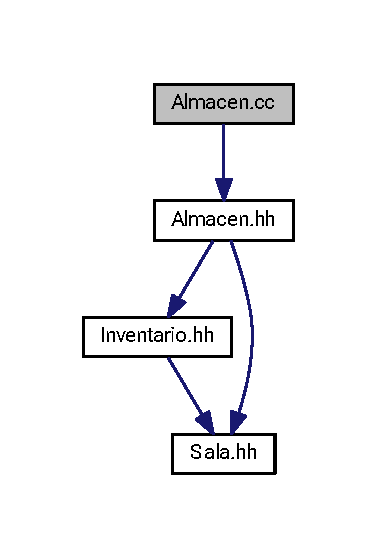
\includegraphics[width=181pt]{_almacen_8cc__incl}
\end{center}
\end{figure}


\subsection{Descripción detallada}
Código de la clase \hyperlink{class_almacen}{Almacen}. 


\hypertarget{_almacen_8hh}{}\section{Referencia del Archivo Almacen.\+hh}
\label{_almacen_8hh}\index{Almacen.\+hh@{Almacen.\+hh}}


Especificación de la clase \hyperlink{class_almacen}{Almacen}.  


Dependencia gráfica adjunta para Almacen.\+hh\+:
\nopagebreak
\begin{figure}[H]
\begin{center}
\leavevmode
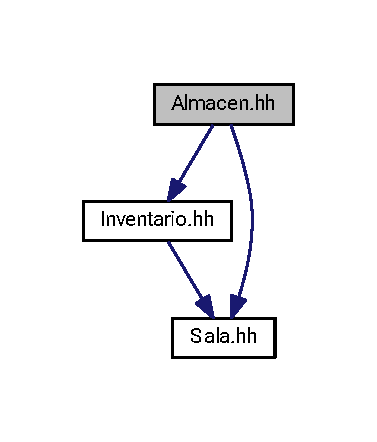
\includegraphics[width=181pt]{_almacen_8hh__incl}
\end{center}
\end{figure}
\subsection*{Clases}
\begin{DoxyCompactItemize}
\item 
class \hyperlink{class_almacen}{Almacen}
\begin{DoxyCompactList}\small\item\em Representa una almacen con varias salas estructuradas en forma de arbol. \end{DoxyCompactList}\end{DoxyCompactItemize}


\subsection{Descripción detallada}
Especificación de la clase \hyperlink{class_almacen}{Almacen}. 


\hypertarget{_inventario_8cc}{}\section{Referencia del Archivo Inventario.\+cc}
\label{_inventario_8cc}\index{Inventario.\+cc@{Inventario.\+cc}}


Código de la clase \hyperlink{class_inventario}{Inventario}.  


Dependencia gráfica adjunta para Inventario.\+cc\+:
\nopagebreak
\begin{figure}[H]
\begin{center}
\leavevmode
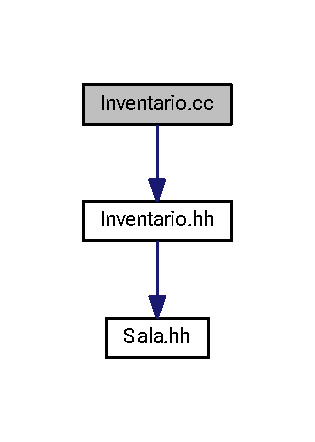
\includegraphics[width=151pt]{_inventario_8cc__incl}
\end{center}
\end{figure}


\subsection{Descripción detallada}
Código de la clase \hyperlink{class_inventario}{Inventario}. 


\hypertarget{_inventario_8hh}{}\section{Referencia del Archivo Inventario.\+hh}
\label{_inventario_8hh}\index{Inventario.\+hh@{Inventario.\+hh}}


Especificación de la clase \hyperlink{class_inventario}{Inventario}.  


Dependencia gráfica adjunta para Inventario.\+hh\+:
\nopagebreak
\begin{figure}[H]
\begin{center}
\leavevmode
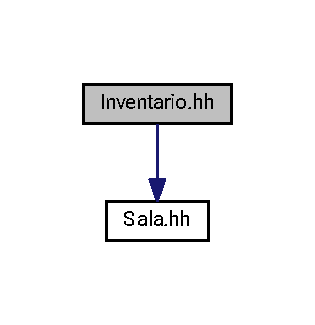
\includegraphics[width=151pt]{_inventario_8hh__incl}
\end{center}
\end{figure}
\subsection*{Clases}
\begin{DoxyCompactItemize}
\item 
class \hyperlink{class_inventario}{Inventario}
\begin{DoxyCompactList}\small\item\em Representa el inventario de los productos de un almacen. \end{DoxyCompactList}\end{DoxyCompactItemize}


\subsection{Descripción detallada}
Especificación de la clase \hyperlink{class_inventario}{Inventario}. 


\hypertarget{program_8cc}{}\section{Referencia del Archivo program.\+cc}
\label{program_8cc}\index{program.\+cc@{program.\+cc}}


Programa principal para la practica {\itshape Tree\+K\+EA}.  


Dependencia gráfica adjunta para program.\+cc\+:
\nopagebreak
\begin{figure}[H]
\begin{center}
\leavevmode
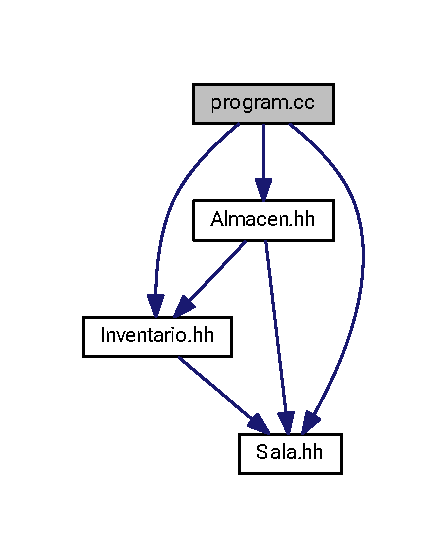
\includegraphics[width=214pt]{program_8cc__incl}
\end{center}
\end{figure}
\subsection*{Funciones}
\begin{DoxyCompactItemize}
\item 
int \hyperlink{program_8cc_ae66f6b31b5ad750f1fe042a706a4e3d4}{main} ()
\begin{DoxyCompactList}\small\item\em Programa principal para la practica {\itshape Tree\+K\+EA}. \end{DoxyCompactList}\end{DoxyCompactItemize}


\subsection{Descripción detallada}
Programa principal para la practica {\itshape Tree\+K\+EA}. 



\subsection{Documentación de las funciones}
\index{program.\+cc@{program.\+cc}!main@{main}}
\index{main@{main}!program.\+cc@{program.\+cc}}
\subsubsection[{\texorpdfstring{main()}{main()}}]{\setlength{\rightskip}{0pt plus 5cm}int main (
\begin{DoxyParamCaption}
{}
\end{DoxyParamCaption}
)}\hypertarget{program_8cc_ae66f6b31b5ad750f1fe042a706a4e3d4}{}\label{program_8cc_ae66f6b31b5ad750f1fe042a706a4e3d4}


Programa principal para la practica {\itshape Tree\+K\+EA}. 

Los datos que se leeran seran siempre correctos respecto al enunciado de la practica. No hay ninguna comprobacion al respecto (ejemplo\+: consultar sala 8 en un almacen de 7 salas). Aqui se leeran y ejecutaran las instrucciones escritas por el usuario. 

Definición en la línea 25 del archivo program.\+cc.


\begin{DoxyCode}
25           \{
26     \textcolor{keywordtype}{int} n;
27     cin>>n;
28     
29     \hyperlink{class_almacen}{Almacen} a (n);
30     a.creabtree();
31     a.inisalas();
32     
33     \hyperlink{class_inventario}{Inventario} inven;
34     
35     \textcolor{keywordtype}{string} op;
36     \textcolor{keywordflow}{while} (cin>>op and op != \textcolor{stringliteral}{"fin"})\{
37         cout << op ;
38         
39         \textcolor{keywordflow}{if} (op == \textcolor{stringliteral}{"poner\_prod"})\{
40             \textcolor{keywordtype}{string} p;
41             cin >> p;
42             cout << \textcolor{stringliteral}{" "} << p << endl;
43             inven.\hyperlink{class_inventario_abe2124eed6c79aca488754a28142a3a6}{poner\_prod}(p);
44         \}
45         
46         \textcolor{keywordflow}{else} \textcolor{keywordflow}{if} (op == \textcolor{stringliteral}{"quitar\_prod"})\{
47             \textcolor{keywordtype}{string} p;
48             cin >> p;
49             cout << \textcolor{stringliteral}{" "} << p << endl;
50             inven.\hyperlink{class_inventario_a7a9da8d5d032fc99b5a423209f871f8b}{quitar\_prod}(p);
51         \}
52         
53         \textcolor{keywordflow}{else} \textcolor{keywordflow}{if} (op == \textcolor{stringliteral}{"poner\_items"})\{
54             \textcolor{keywordtype}{int} id,cant;
55             \textcolor{keywordtype}{string} prod;
56             cin >> \textcolor{keywordtype}{id} >> prod >> cant;
57             cout << \textcolor{stringliteral}{" "} << \textcolor{keywordtype}{id} << \textcolor{stringliteral}{" "}<< prod << \textcolor{stringliteral}{" "} << cant << endl;
58             a.poner\_items(\textcolor{keywordtype}{id}, prod, cant, inven);
59         \}
60         
61         \textcolor{keywordflow}{else} \textcolor{keywordflow}{if} (op == \textcolor{stringliteral}{"quitar\_items"})\{
62             \textcolor{keywordtype}{int} id,cant;
63             \textcolor{keywordtype}{string} prod;
64             cin >> \textcolor{keywordtype}{id} >> prod >> cant;
65             cout << \textcolor{stringliteral}{" "} << \textcolor{keywordtype}{id} << \textcolor{stringliteral}{" "} << prod << \textcolor{stringliteral}{" "} << cant << endl;
66             a.quitar\_items(\textcolor{keywordtype}{id}, prod, cant, inven);
67         \}
68         
69         \textcolor{keywordflow}{else} \textcolor{keywordflow}{if} (op == \textcolor{stringliteral}{"distribuir"})\{
70             \textcolor{keywordtype}{string} prod;
71             \textcolor{keywordtype}{int} cant;
72             cin >> prod >> cant;
73             cout << \textcolor{stringliteral}{" "} << prod << \textcolor{stringliteral}{" "} << cant << endl;
74             a.distribuir(prod, cant, inven);
75         \}
76         
77         \textcolor{keywordflow}{else} \textcolor{keywordflow}{if} (op == \textcolor{stringliteral}{"compactar"})\{
78             \textcolor{keywordtype}{int} id;
79             cin >> id;
80             cout << \textcolor{stringliteral}{" "} << \textcolor{keywordtype}{id} << endl;
81             a.compactar(\textcolor{keywordtype}{id});
82         \}
83         
84         \textcolor{keywordflow}{else} \textcolor{keywordflow}{if} (op == \textcolor{stringliteral}{"reorganizar"})\{
85             \textcolor{keywordtype}{int} id;
86             cin >> id;
87             cout <<  \textcolor{stringliteral}{" "} << \textcolor{keywordtype}{id} << endl;
88             a.reorganizar(\textcolor{keywordtype}{id});
89         \}
90         
91         \textcolor{keywordflow}{else} \textcolor{keywordflow}{if} (op == \textcolor{stringliteral}{"redimensionar"})\{
92             \textcolor{keywordtype}{int} id, f, c;
93             cin >> \textcolor{keywordtype}{id} >> f >> c;
94             cout << \textcolor{stringliteral}{" "} << \textcolor{keywordtype}{id} << \textcolor{stringliteral}{" "} << f << \textcolor{stringliteral}{" "} << c << endl;
95             a.redimensionar(\textcolor{keywordtype}{id}, f ,c);
96         \}
97         
98         \textcolor{keywordflow}{else} \textcolor{keywordflow}{if} (op == \textcolor{stringliteral}{"inventario"})\{
99             cout << endl;
100             inven.\hyperlink{class_inventario_aa764715a4df95aed453d73a8d509e344}{consultar\_inven}();
101         \}
102         
103         \textcolor{keywordflow}{else} \textcolor{keywordflow}{if} (op == \textcolor{stringliteral}{"escribir"})\{
104             \textcolor{keywordtype}{int} id;
105             cin>>id;
106             cout<< \textcolor{stringliteral}{" "} << \textcolor{keywordtype}{id} << endl;
107             a.escribir(\textcolor{keywordtype}{id});
108         \}
109         
110         \textcolor{keywordflow}{else} \textcolor{keywordflow}{if} (op == \textcolor{stringliteral}{"consultar\_pos"})\{
111             \textcolor{keywordtype}{int} id, f ,c;
112             cin >> \textcolor{keywordtype}{id} >> f >> c;
113             cout << \textcolor{stringliteral}{" "} << \textcolor{keywordtype}{id} << \textcolor{stringliteral}{" "}<< f << \textcolor{stringliteral}{" "} << c <<endl;
114             a.consultar\_pos(\textcolor{keywordtype}{id}, f, c);
115         \}
116         
117         \textcolor{keywordflow}{else} \textcolor{keywordflow}{if} (op == \textcolor{stringliteral}{"consultar\_prod"})\{
118             \textcolor{keywordtype}{string} prod;
119             cin >> prod;
120             cout << \textcolor{stringliteral}{" "} << prod << endl;
121             inven.\hyperlink{class_inventario_aa8c8b617c44b44819e9dcae3894eeecc}{consultar\_prod}(prod);
122         \}
123     \}
124     
125     cout << op << endl;
126 \}
\end{DoxyCode}

\hypertarget{_sala_8cc}{}\section{Referencia del Archivo Sala.\+cc}
\label{_sala_8cc}\index{Sala.\+cc@{Sala.\+cc}}


Código de la clase \hyperlink{class_sala}{Sala}.  


Dependencia gráfica adjunta para Sala.\+cc\+:
\nopagebreak
\begin{figure}[H]
\begin{center}
\leavevmode
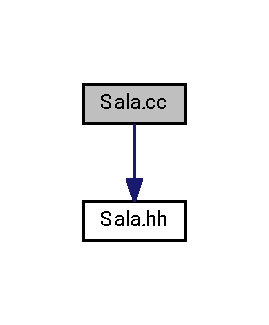
\includegraphics[width=129pt]{_sala_8cc__incl}
\end{center}
\end{figure}


\subsection{Descripción detallada}
Código de la clase \hyperlink{class_sala}{Sala}. 


\hypertarget{_sala_8hh}{}\section{Referencia del Archivo Sala.\+hh}
\label{_sala_8hh}\index{Sala.\+hh@{Sala.\+hh}}


Especificación de la clase \hyperlink{class_sala}{Sala}.  


\subsection*{Clases}
\begin{DoxyCompactItemize}
\item 
class \hyperlink{class_sala}{Sala}
\begin{DoxyCompactList}\small\item\em Representa una sala de un numero de filas y columnas. \end{DoxyCompactList}\end{DoxyCompactItemize}


\subsection{Descripción detallada}
Especificación de la clase \hyperlink{class_sala}{Sala}. 


%--- End generated contents ---

% Index
\backmatter
\newpage
\phantomsection
\clearemptydoublepage
\addcontentsline{toc}{chapter}{Índice}
\printindex

\end{document}
